\documentclass{article}

% Preamble: Package Loading
\usepackage[fleqn]{amsmath}
\usepackage{amsfonts}
\usepackage{amssymb}
\usepackage{ctex}
\usepackage{graphicx}
\usepackage{CJKutf8}
\usepackage{tikz}
\usepackage{geometry}
\usepackage{epsfig}
\usepackage{epstopdf}

% Document Geometry
\geometry{a4paper, margin=1in}

\begin{document}
	
	\title{数学物理方法笔记 (Fourier Analysis Notes)}
	\author{Darryl}
	\date{\today}
	\maketitle
	
	%====================================================================
	\section{傅立叶级数 (Fourier Series)}
	%====================================================================
	
	\subsection{一般理论 (General Theory)}
	给定一个周期为 $2L$ 的函数 $f(x)$,即 $f(x+2L) = f(x)$,其傅立叶级数展开为:
	$$ 
	f(x) = a_0 + \sum_{n=1}^{\infty} (a_n \cos(\frac{n\pi x}{L}) + b_n \sin(\frac{n\pi x}{L})) 
	$$
	其中系数由以下积分给出:
	\begin{align*}
		a_0 &= \frac{1}{2L} \int_{-L}^{L} f(t) dt \\
		a_n &= \frac{1}{L} \int_{-L}^{L} f(t) \cos(\frac{n\pi t}{L}) dt \\
		b_n &= \frac{1}{L} \int_{-L}^{L} f(t) \sin(\frac{n\pi t}{L}) dt
	\end{align*}
	
	对于周期为 $2\pi$ 的函数(即 $L=\pi$):
	$$ 
	f(x) = a_0 + \sum_{n=1}^{\infty} (a_n \cos(nx) + b_n \sin(nx)) 
	$$
	通过在 $[0, 2\pi]$ 上积分可以推导出系数:
	$$ 
	\int_0^{2\pi} f(x) dx = \int_0^{2\pi} \left[a_0 + \sum_{n=1}^{\infty} (a_n \cos(nx) + b_n \sin(nx))\right] dx = 2\pi a_0 
	$$
	$$ 
	\Rightarrow a_0 = \frac{1}{2\pi} \int_0^{2\pi} f(x) dx 
	$$
	利用三角函数的正交性:
	$$ 
	\int_0^{2\pi} f(x) \cos(mx) dx = \sum_{n=1}^{\infty} a_n \int_0^{2\pi} \cos(nx)\cos(mx)dx = a_m \pi 
	$$
	$$ 
	\Rightarrow a_n = \frac{1}{\pi} \int_0^{2\pi} f(x) \cos(nx) dx 
	$$
	同理可得 $b_n$:
	$$ 
	\Rightarrow b_n = \frac{1}{\pi} \int_0^{2\pi} f(x) \sin(nx) dx 
	$$
	
	\paragraph{狄利克雷定理 (Dirichlet's Theorem):}
	如果 $f(x)$ 在 $[-L, L]$ 上除有限个点外连续,且有有限个极值点。在 $(-L, L)$ 外为周期延拓,周期为 $2L$。则 $f(x)$ 的傅立叶级数收敛于:
	$$ 
	\frac{f(x+0) + f(x-0)}{2} 
	$$
	
	\subsection{正交函数系展开 (Expansion in Orthogonal Function Systems)}
	\paragraph{正弦级数 (Sine Series):}
	若函数 $\phi(x)$ 在 $(0, L)$ 上展开为正弦级数:
	$$ 
	\phi(x) = \sum_{n=1}^{\infty} C_n \sin\left(\frac{n\pi x}{L}\right), \quad 0 < x < L 
	$$
	利用正交关系 $\int_0^L \sin\left(\frac{m\pi x}{L}\right) \sin\left(\frac{n\pi x}{L}\right) dx = \frac{L}{2}\delta_{mn}$,可得系数:
	$$ 
	\int_0^L \phi(x) \sin\left(\frac{m\pi x}{L}\right) dx = C_m \frac{L}{2} 
	$$
	$$ 
	\Rightarrow C_n = \frac{2}{L} \int_0^L \phi(x) \sin\left(\frac{n\pi x}{L}\right) dx 
	$$
	
	\paragraph{余弦级数 (Cosine Series):}
	若函数 $\phi(x)$ 在 $(0, L)$ 上展开为余弦级数:
	$$ 
	\phi(x) = D_0 + \sum_{n=1}^{\infty} D_n \cos\left(\frac{n\pi x}{L}\right) 
	$$
	利用正交关系可得系数:
	$$ 
	D_0 = \frac{1}{L} \int_0^L \phi(x) dx 
	$$
	$$ 
	D_n = \frac{2}{L} \int_0^L \phi(x) \cos\left(\frac{n\pi x}{L}\right) dx 
	$$
	
	\subsection{傅立叶级数示例 (Fourier Series Examples)}
	\paragraph{例1:} $f(x) = \frac{1}{2}(\pi-x)$ on $(0, 2\pi)$, with $f(x+2\pi) = f(x)$.
	\begin{align*}
		a_0 &= \frac{1}{2\pi} \int_0^{2\pi} \frac{1}{2}(\pi-x) dx = 0 \\
		a_n &= \frac{1}{\pi} \int_0^{2\pi} \frac{1}{2}(\pi-x) \cos(nx) dx = 0 \\
		b_n &= \frac{1}{\pi} \int_0^{2\pi} \frac{1}{2}(\pi-x) \sin(nx) dx \\
		&= \frac{1}{2\pi} \left[ (\pi-x) \left(-\frac{\cos(nx)}{n}\right) \right]_0^{2\pi} - \frac{1}{2\pi} \int_0^{2\pi} (-1) \left(-\frac{\cos(nx)}{n}\right) dx \\
		&= \frac{1}{2\pi} \left[ \frac{\pi}{n} + \frac{\pi}{n} \right] - 0 = \frac{1}{n}
	\end{align*}
	所以:
	$$ 
	f(x) = \sum_{n=1}^{\infty} \frac{\sin(nx)}{n} 
	$$
	
	\paragraph{例2:} 将 $\phi(x) = \sin x$ 在 $[0, \pi]$ 上展开为余弦级数。这里 $L=\pi$。
	\begin{align*}
		D_0 &= \frac{1}{\pi} \int_0^\pi \sin x \, dx = \frac{1}{\pi} [-\cos x]_0^\pi = \frac{2}{\pi} \\
		D_n &= \frac{2}{\pi} \int_0^\pi \sin x \cos(nx) \, dx = \frac{1}{\pi} \int_0^\pi [\sin((1+n)x) + \sin((1-n)x)] \, dx \\
		&= \frac{1}{\pi} \left[ -\frac{\cos((1+n)x)}{1+n} - \frac{\cos((1-n)x)}{1-n} \right]_0^\pi \quad (n \ne 1) \\
		&= \frac{1}{\pi} \left( \frac{1-\cos((n+1)\pi)}{n+1} + \frac{1-\cos((n-1)\pi)}{n-1} \right) \\
		&= \frac{1}{\pi} \left( \frac{1-(-1)^{n+1}}{n+1} + \frac{1-(-1)^{n-1}}{n-1} \right) = \frac{1+(-1)^n}{\pi} \left( \frac{1}{n+1} + \frac{1}{n-1} \right) \\
		&= \frac{2(1+(-1)^n)}{\pi(n^2-1)}
	\end{align*}
	当 $n=1$ 时, $D_1 = \frac{2}{\pi} \int_0^\pi \sin x \cos x \, dx = 0$。\\
	$D_n$ 仅在 $n$ 为偶数时非零。令 $n=2k$:
	$$ 
	D_{2k} = \frac{4}{\pi((2k)^2-1)} 
	$$
	所以:
	$$ 
	\phi(x) = \frac{2}{\pi} + \sum_{k=1}^{\infty} \frac{4}{\pi(1-(2k)^2)} \cos(2kx) = \frac{2}{\pi} - \frac{4}{\pi} \sum_{k=1}^{\infty} \frac{\cos(2kx)}{4k^2-1} 
	$$
	
	%====================================================================
	\section{傅立叶积分 (Fourier Integral)}
	%====================================================================
	\subsection{从级数到积分 (From Series to Integral)}
	考虑傅立叶级数,当 $L \to \infty$ 时,$\omega_n = \frac{n\pi}{L}$, $\Delta\omega = \omega_{n+1} - \omega_n = \frac{\pi}{L}$。
	级数求和变为积分: $\sum_{n=1}^\infty \to \frac{L}{\pi} \sum \Delta\omega \to \frac{1}{\pi} \int_0^\infty d\omega$。
	$$ 
	f(x) = \int_0^\infty [A(\omega)\cos(\omega x) + B(\omega)\sin(\omega x)] d\omega 
	$$
	其中系数为:
	\begin{align*}
		A(\omega) &= \frac{1}{\pi} \int_{-\infty}^{\infty} f(t) \cos(\omega t) dt \\
		B(\omega) &= \frac{1}{\pi} \int_{-\infty}^{\infty} f(t) \sin(\omega t) dt
	\end{align*}
	
	\subsection{傅立叶积分示例 (Fourier Integral Examples)}
	\paragraph{例3:} $f(x) = \begin{cases} 1 & |x| \le 1 \\ 0 & |x| > 1 \end{cases}$
	函数为偶函数,所以 $B(\omega)=0$。
	$$ 
	A(\omega) = \frac{1}{\pi} \int_{-\infty}^\infty f(t)\cos(\omega t) dt = \frac{1}{\pi} \int_{-1}^1 \cos(\omega t) dt = \frac{1}{\pi} \left[\frac{\sin(\omega t)}{\omega}\right]_{-1}^1 = \frac{2\sin\omega}{\pi\omega} 
	$$
	所以:
	$$ 
	f(x) = \int_0^\infty \frac{2\sin\omega}{\pi\omega} \cos(\omega x) d\omega = \frac{2}{\pi} \int_0^\infty \frac{\sin\omega \cos(\omega x)}{\omega} d\omega 
	$$
	
	\paragraph{例4:} $f(x) = \begin{cases} \cos x & |x| \le \frac{\pi}{2} \\ 0 & |x| > \frac{\pi}{2} \end{cases}$
	函数为偶函数,所以 $B(\omega)=0$。
	\begin{align*}
		A(\omega) &= \frac{1}{\pi} \int_{-\pi/2}^{\pi/2} \cos t \cos(\omega t) dt = \frac{2}{\pi} \int_0^{\pi/2} \cos t \cos(\omega t) dt \\
		&= \frac{1}{\pi} \int_0^{\pi/2} [\cos((1+\omega)t) + \cos((1-\omega)t)] dt \\
		&= \frac{1}{\pi} \left[ \frac{\sin((1+\omega)t)}{1+\omega} + \frac{\sin((1-\omega)t)}{1-\omega} \right]_0^{\pi/2} \quad (\omega \ne 1) \\
		&= \frac{1}{\pi} \left( \frac{\sin(\frac{\pi}{2}(1+\omega))}{1+\omega} + \frac{\sin(\frac{\pi}{2}(1-\omega))}{1-\omega} \right) \\
		&= \frac{1}{\pi} \left( \frac{\cos(\frac{\pi\omega}{2})}{1+\omega} + \frac{\cos(\frac{\pi\omega}{2})}{1-\omega} \right) = \frac{2\cos(\frac{\pi\omega}{2})}{\pi(1-\omega^2)}
	\end{align*}
	所以:
	$$ 
	f(x) = \frac{2}{\pi} \int_0^\infty \frac{\cos(\frac{\pi\omega}{2})}{1-\omega^2} \cos(\omega x) d\omega 
	$$
	
	%====================================================================
	\section{复数形式的傅立叶变换 (Complex Form and Fourier Transform)}
	%====================================================================
	傅立叶积分可以写为:
	\begin{align*}
		f(x) &= \frac{1}{\pi} \int_0^\infty d\omega \int_{-\infty}^\infty f(t) \cos(\omega(x-t)) dt \\
		&= \frac{1}{2\pi} \int_0^\infty d\omega \int_{-\infty}^\infty f(t) [e^{i\omega(x-t)} + e^{-i\omega(x-t)}] dt \\
		&= \frac{1}{2\pi} \int_{-\infty}^\infty d\omega \int_{-\infty}^\infty f(t) e^{i\omega(x-t)} dt
	\end{align*}
	这引出了傅立叶变换对:
	\begin{align*}
		\text{傅立叶变换 (Fourier Transform):} & \quad F(\omega) = \int_{-\infty}^\infty f(x) e^{-i\omega x} dx \\
		\text{傅立叶逆变换 (Inverse F.T.):} & \quad f(x) = \frac{1}{2\pi} \int_{-\infty}^\infty F(\omega) e^{i\omega x} d\omega
	\end{align*}
	
	\subsection{傅立叶变换示例 (Fourier Transform Example)}
	\paragraph{例4 (续):} $f(x) = \begin{cases} 1 & |x| < a \\ 0 & |x| > a \end{cases}$
	\begin{align*}
		F(\omega) &= \int_{-\infty}^\infty f(x) e^{-i\omega x} dx = \int_{-a}^a 1 \cdot e^{-i\omega x} dx \\
		&= \left[ \frac{e^{-i\omega x}}{-i\omega} \right]_{-a}^a = \frac{e^{-i\omega a} - e^{i\omega a}}{-i\omega} = \frac{2\sin(\omega a)}{\omega}
	\end{align*}
	通过逆变换得到傅立叶积分表示:
	\begin{align*}
		f(x) &= \frac{1}{2\pi} \int_{-\infty}^\infty F(\omega) e^{i\omega x} d\omega = \frac{1}{2\pi} \int_{-\infty}^\infty \frac{2\sin(\omega a)}{\omega} e^{i\omega x} d\omega \\
		&= \frac{1}{\pi} \int_{-\infty}^\infty \frac{\sin(\omega a)}{\omega} (\cos(\omega x) + i\sin(\omega x)) d\omega
	\end{align*}
	由于 $\frac{\sin(\omega a)}{\omega}\sin(\omega x)$ 是奇函数,其积分为零。
	$$ 
	f(x) = \frac{1}{\pi} \int_{-\infty}^\infty \frac{\sin(\omega a)\cos(\omega x)}{\omega} d\omega = \frac{2}{\pi} \int_0^\infty \frac{\sin(\omega a)\cos(\omega x)}{\omega} d\omega 
	$$
	根据收敛定理,该积分等于:
	$$ 
	\begin{cases} 1 & |x| < a \\ 1/2 & |x| = a \\ 0 & |x| > a \end{cases} 
	$$
	
	%====================================================================
	\section{傅立叶变换性质 (Properties of Fourier Transform)}
	%====================================================================
	令 $F(\omega)$ 是 $f(x)$ 的傅立叶变换, $F(\omega) = \mathcal{F}[f(x)] = \int_{-\infty}^{\infty} f(x) e^{-i\omega x} dx$.
	
	\begin{enumerate}
		\item \textbf{导数 (Differentiation):}
		$$ \mathcal{F}\left[\frac{df(x)}{dx}\right] = i\omega F(\omega) $$
		推导:
		\begin{align*}
			\int_{-\infty}^{\infty} \frac{df(x)}{dx} e^{-i\omega x} dx &= \left[ f(x) e^{-i\omega x} \right]_{-\infty}^{\infty} - \int_{-\infty}^{\infty} f(x) (-i\omega) e^{-i\omega x} dx \\
			&= 0 + i\omega \int_{-\infty}^{\infty} f(x) e^{-i\omega x} dx = i\omega F(\omega)
		\end{align*}
		
		\item \textbf{乘以 $x$ (Multiplication by $x$):}
		$$ \mathcal{F}[x f(x)] = i \frac{dF(\omega)}{d\omega} $$
		推导:
		$$ \frac{dF(\omega)}{d\omega} = \frac{d}{d\omega} \int_{-\infty}^{\infty} f(x) e^{-i\omega x} dx = \int_{-\infty}^{\infty} -ix f(x) e^{-i\omega x} dx = -i \mathcal{F}[x f(x)] $$
		推广可得:
		$$ \mathcal{F}[x^n f(x)] = i^n \frac{d^n F(\omega)}{d\omega^n} $$
		
		\item \textbf{积分 (Integration):}
		若 $g(x) = \int_{-\infty}^x f(\xi) d\xi$, 且 $f(x)=g'(x)$, 则
		$$ F(\omega) = \mathcal{F}[g'(x)] = i\omega G(\omega) $$
		$$ G(\omega) = \mathcal{F}\left[\int_{-\infty}^x f(\xi)d\xi\right] = \frac{1}{i\omega}F(\omega) \quad (\text{可能需要加上 } \pi F(0)\delta(\omega) \text{ 项})$$
		
		\item \textbf{位移 (Shifting):}
		$$ \mathcal{F}[f(x+\xi)] = e^{i\omega\xi} F(\omega) $$
		推导 (令 $y=x+\xi$):
		$$ \int_{-\infty}^{\infty} f(x+\xi) e^{-i\omega x} dx = \int_{-\infty}^{\infty} f(y) e^{-i\omega(y-\xi)} dy = e^{i\omega\xi} \int_{-\infty}^{\infty} f(y) e^{-i\omega y} dy = e^{i\omega\xi} F(\omega) $$
		
		\item \textbf{卷积 (Convolution):}
		卷积定义: $f_1(x) * f_2(x) = \int_{-\infty}^{\infty} f_1(\xi) f_2(x-\xi) d\xi$.
		$$ \mathcal{F}[f_1 * f_2] = F_1(\omega) F_2(\omega) $$
		推导:
		\begin{align*}
			\mathcal{F}[f_1 * f_2] &= \int_{-\infty}^{\infty} \left[ \int_{-\infty}^{\infty} f_1(\xi) f_2(x-\xi) d\xi \right] e^{-i\omega x} dx \\
			&= \int_{-\infty}^{\infty} f_1(\xi) \left[ \int_{-\infty}^{\infty} f_2(x-\xi) e^{-i\omega x} dx \right] d\xi \\
			\text{(令 } y=x-\xi \text{)} &= \int_{-\infty}^{\infty} f_1(\xi) \left[ \int_{-\infty}^{\infty} f_2(y) e^{-i\omega(y+\xi)} dy \right] d\xi \\
			&= \left( \int_{-\infty}^{\infty} f_1(\xi) e^{-i\omega\xi} d\xi \right) \left( \int_{-\infty}^{\infty} f_2(y) e^{-i\omega y} dy \right) = F_1(\omega) F_2(\omega)
		\end{align*}
	\end{enumerate}
	
	%====================================================================
	\section{狄拉克 $\delta$ 函数 (Dirac Delta Function)}
	%====================================================================
	\subsection{定义与性质 (Definition and Properties)}
	$\delta$ 函数定义为满足以下条件的分布:
	$$ 
	\delta(x-x_0) = \begin{cases} 0 & x \ne x_0 \\ \infty & x = x_0 \end{cases} \quad \text{且} \quad \int_{-\infty}^{\infty} \delta(x-x_0) dx = 1 
	$$
	\textbf{筛选性质 (Sifting Property):}
	$$ 
	\int_{-\infty}^{\infty} f(x) \delta(x-x_0) dx = f(x_0) 
	$$
	$\delta(x-x_1)$ 为偶函数, 即 $\delta(x) = \delta(-x)$。
	
	\textbf{卷积性质 (Convolution Properties):}
	\begin{align*}
		\delta(x) * f(x) &= \int_{-\infty}^{\infty} f(\xi) \delta(x-\xi) d\xi = f(x) \\
		\delta(x-a) * f(x) &= f(x-a) \\
		\delta(x-a) * \delta(x-b) &= \delta(x-(a+b))
	\end{align*}
	
	\textbf{傅立叶变换 (Fourier Transform):}
	$$ 
	\mathcal{F}[\delta(x-x_0)] = \int_{-\infty}^{\infty} \delta(x-x_0) e^{-i\omega x} dx = e^{-i\omega x_0} 
	$$
	特别地, 当 $x_0=0$ 时, $\mathcal{F}[\delta(x)] = 1$。
	反变换给出 $\delta$ 函数的一个积分表示:
	$$ 
	\delta(x) = \frac{1}{2\pi} \int_{-\infty}^{\infty} e^{i\omega x} d\omega 
	$$
	
	\subsection{$\delta$ 函数的极限表示 (Limit Representations of $\delta$-Function)}
	\begin{enumerate}
		\item \textbf{Sinc 函数:}
		$$ \delta(x) = \lim_{B\to\infty} \frac{\sin(Bx)}{\pi x} $$
		这来自一个带宽为 $[-B, B]$ 的理想低通滤波器的冲激响应。
		$$ \frac{1}{2\pi} \int_{-B}^{B} e^{i\omega x} d\omega = \frac{\sin(Bx)}{\pi x} $$
		
		\item \textbf{洛伦兹函数 (Lorentzian Function):}
		$$ \delta(x) = \lim_{b\to 0^+} \frac{1}{\pi} \frac{b}{x^2+b^2} $$
		
		\item \textbf{狄利克雷核 (Dirichlet Kernel, 在周期区间上):}
		$$ \sum_{k=-\infty}^{\infty} \delta(x-2\pi k) = \frac{1}{2\pi} \lim_{m\to\infty} D_m(x) = \frac{1}{2\pi} \lim_{m\to\infty} \sum_{n=-m}^{m} e^{inx} $$
		其中 $D_m(x) = 1 + 2\sum_{n=1}^m \cos(nx) = \frac{\sin((m+1/2)x)}{\sin(x/2)}$。
	\end{enumerate}
	
	%====================================================================
	\section{傅立叶级数的收敛与狄利克雷核}
	%====================================================================
	\subsection{部分和 (Partial Sum)}
	傅立叶级数的部分和 $S_m(x)$ 可以表示为与狄利克雷核的卷积:
	\begin{align*}
		S_m(x) &= \frac{a_0}{2} + \sum_{n=1}^{m} (a_n \cos(nx) + b_n \sin(nx)) \\
		&= \frac{1}{2\pi} \int_{-\pi}^{\pi} f(t) dt + \sum_{n=1}^{m} \frac{1}{\pi} \int_{-\pi}^{\pi} f(t) \cos(n(t-x)) dt \\
		&= \frac{1}{\pi} \int_{-\pi}^{\pi} f(t) \left[ \frac{1}{2} + \sum_{n=1}^{m} \cos(n(t-x)) \right] dt \\
		&= \frac{1}{2\pi} \int_{-\pi}^{\pi} f(t) D_m(t-x) dt
	\end{align*}
	其中 $D_m(u) = \sum_{n=-m}^{m} e^{inu} = \frac{\sin((m+1/2)u)}{\sin(u/2)}$ 是狄利克雷核。
	令 $u = t-x$, 并利用周期性:
	$$ 
	S_m(x) = \frac{1}{2\pi} \int_{-\pi}^{\pi} f(x+u) D_m(u) du 
	$$
	由于 $D_m(u)$ 是偶函数,
	$$ 
	S_m(x) = \frac{1}{2\pi} \int_0^{\pi} [f(x+u) + f(x-u)] D_m(u) du 
	$$
	
	\subsection{收敛证明概要 (Sketch of Convergence Proof)}
	利用狄利克雷核的性质 $\frac{1}{2\pi} \int_{-\pi}^{\pi} D_m(u) du = 1$, 可得
	$$ 
	\frac{f(x+0) + f(x-0)}{2} = \frac{1}{2\pi} \int_0^{\pi} [f(x+0) + f(x-0)] D_m(u) du 
	$$
	考虑差值:
	$$ 
	S_m(x) - \frac{f(x+0) + f(x-0)}{2} = \frac{1}{2\pi} \int_0^{\pi} [f(x+u) - f(x+0) + f(x-u) - f(x-0)] D_m(u) du 
	$$
	$$ 
	= \frac{1}{2\pi} \int_0^{\pi} \left[ \frac{f(x+u) - f(x+0)}{u} + \frac{f(x-u) - f(x-0)}{u} \right] u \frac{\sin((m+1/2)u)}{\sin(u/2)} du 
	$$
	当 $f(x)$ 满足狄利克雷条件时, 方括号内的函数在 $[0, \pi]$ 上绝对可积。根据黎曼-勒贝格引理 (Riemann-Lebesgue Lemma), 当 $m \to \infty$ 时, 该积分趋于零。
	因此, $\lim_{m\to\infty} S_m(x) = \frac{f(x+0) + f(x-0)}{2}$。
	
	%====================================================================
	\section{更多傅立叶变换示例 (More Fourier Transform Examples)}
	%====================================================================
	
	\subsection{高斯函数 (Gaussian Function)}
	\paragraph{例:} 求 $f(x) = e^{-ax^2}$ (其中 $a>0$) 的傅立叶变换。
	\begin{align*}
		G(\omega) &= \mathcal{F}[e^{-ax^2}] = \int_{-\infty}^{\infty} e^{-ax^2} e^{-i\omega x} dx \\
		&= \int_{-\infty}^{\infty} e^{-(ax^2 + i\omega x)} dx
	\end{align*}
	为了求解这个积分,我们使用配方法:
	$$ 
	ax^2 + i\omega x = a\left(x^2 + \frac{i\omega}{a}x\right) = a\left(x + \frac{i\omega}{2a}\right)^2 - a\left(\frac{i\omega}{2a}\right)^2 = a\left(x + \frac{i\omega}{2a}\right)^2 + \frac{\omega^2}{4a} 
	$$
	代入积分中可得:
	\begin{align*}
		G(\omega) &= \int_{-\infty}^{\infty} \exp\left[-a\left(x + \frac{i\omega}{2a}\right)^2 - \frac{\omega^2}{4a}\right] dx \\
		&= e^{-\frac{\omega^2}{4a}} \int_{-\infty}^{\infty} e^{-a\left(x + \frac{i\omega}{2a}\right)^2} dx
	\end{align*}
	令 $y = \sqrt{a}(x + \frac{i\omega}{2a})$, $dy = \sqrt{a}dx$。这是一个在复平面上的积分,但可以证明其路径可以平移回实轴而不改变积分值。因此,积分结果等于标准高斯积分 $\int_{-\infty}^\infty e^{-y^2} dy = \sqrt{\pi}$。
	$$ 
	G(\omega) = e^{-\frac{\omega^2}{4a}} \cdot \frac{1}{\sqrt{a}} \int_{-\infty}^{\infty} e^{-y^2} dy = \sqrt{\frac{\pi}{a}} e^{-\frac{\omega^2}{4a}} 
	$$
	这是一个非常重要的结论:**高斯函数的傅立叶变换仍然是高斯函数**。
	
	\paragraph{应用:} 利用傅立叶逆变换,我们可以求解一个重要的积分。
	$$ 
	f(x) = e^{-ax^2} = \frac{1}{2\pi} \int_{-\infty}^{\infty} G(\omega) e^{i\omega x} d\omega = \frac{1}{2\pi} \int_{-\infty}^{\infty} \sqrt{\frac{\pi}{a}} e^{-\frac{\omega^2}{4a}} e^{i\omega x} d\omega 
	$$
	$$ 
	\Rightarrow \int_{-\infty}^{\infty} e^{-\frac{\omega^2}{4a}} (\cos(\omega x) + i\sin(\omega x)) d\omega = 2\pi \sqrt{\frac{a}{\pi}} e^{-ax^2} = \sqrt{4\pi a} e^{-ax^2} 
	$$
	取等式两边的实部,并设 $a=1/4$,则有:
	$$ 
	\int_{-\infty}^{\infty} e^{-\omega^2} \cos(\omega x) d\omega = \sqrt{\pi} e^{-x^2/4} 
	$$
	
	\subsection{基本函数 (Basic Functions)}
	\paragraph{例:$f(x) = \sin(kx)$}
	\begin{align*}
		\mathcal{F}[\sin(kx)] &= \int_{-\infty}^{\infty} \frac{e^{ikx}-e^{-ikx}}{2i} e^{-i\omega x} dx \\
		&= \frac{1}{2i} \left[ \int_{-\infty}^{\infty} e^{-i(\omega-k)x} dx - \int_{-\infty}^{\infty} e^{-i(\omega+k)x} dx \right] \\
		&= \frac{1}{2i} [2\pi \delta(\omega-k) - 2\pi \delta(\omega+k)] \\
		&= i\pi [\delta(\omega+k) - \delta(\omega-k)]
	\end{align*}
	
	\paragraph{例:$f(x) = e^{-|x|}$}
	\begin{align*}
		F(\omega) &= \int_{-\infty}^{\infty} e^{-|x|} e^{-i\omega x} dx = \int_{-\infty}^{0} e^{x} e^{-i\omega x} dx + \int_{0}^{\infty} e^{-x} e^{-i\omega x} dx \\
		&= \int_{-\infty}^{0} e^{(1-i\omega)x} dx + \int_{0}^{\infty} e^{-(1+i\omega)x} dx \\
		&= \left[ \frac{e^{(1-i\omega)x}}{1-i\omega} \right]_{-\infty}^0 + \left[ \frac{e^{-(1+i\omega)x}}{-(1+i\omega)} \right]_0^{\infty} \\
		&= \frac{1}{1-i\omega} + \frac{1}{1+i\omega} = \frac{1+i\omega+1-i\omega}{1+\omega^2} = \frac{2}{1+\omega^2}
	\end{align*}
	通过傅立叶逆变换:
	$$ 
	f(x) = e^{-|x|} = \frac{1}{2\pi} \int_{-\infty}^{\infty} \frac{2}{1+\omega^2} e^{i\omega x} d\omega = \frac{1}{\pi} \int_{-\infty}^{\infty} \frac{\cos(\omega x)}{1+\omega^2} d\omega 
	$$
	
	\subsection{双曲正割与三角脉冲 (Hyperbolic Secant and Triangular Pulse)}
	
	\paragraph{例:$f(x) = \text{sech}(kx)$}
	其傅立叶变换为:
	$$ 
	F(\omega) = \mathcal{F}[\text{sech}(kx)] = \frac{\pi}{k} \text{sech}\left(\frac{\pi\omega}{2k}\right) 
	$$
	
	\paragraph{例:三角脉冲函数}
	$f(x) = \Delta(x) = \begin{cases} 1-|x| & |x| \le 1 \\ 0 & |x| > 1 \end{cases}$
	\begin{align*}
		F(\omega) &= \int_{-1}^{1} (1-|x|) e^{-i\omega x} dx = \int_{-1}^{0} (1+x)e^{-i\omega x}dx + \int_{0}^{1} (1-x)e^{-i\omega x}dx \\
		&= \dots \quad (\text{通过两次分部积分}) \\
		&= \frac{2(1-\cos\omega)}{\omega^2} = \frac{4\sin^2(\omega/2)}{\omega^2} = \left(\frac{\sin(\omega/2)}{\omega/2}\right)^2
	\end{align*}
	
	%====================================================================
	\section{赫维赛德阶跃函数的变换 (Transform of Heaviside Step Function)}
	%====================================================================
	赫维赛德阶跃函数 $u(t)$ 的傅立叶变换需要通过极限过程来定义。我们首先考虑一个单边指数衰减函数 $f(t) = e^{-Bt}u(t)$, 其中 $B>0$。
	$$ 
	\mathcal{F}[e^{-Bt}u(t)] = \int_0^{\infty} e^{-Bt} e^{-i\omega t} dt = \int_0^{\infty} e^{-(B+i\omega)t} dt = \frac{1}{B+i\omega} 
	$$
	现在我们令 $B \to 0^+$,来得到阶跃函数的变换:
	$$ 
	\mathcal{F}[u(t)] = \lim_{B\to 0^+} \frac{1}{B+i\omega} 
	$$
	这个极限在分布意义下等于:
	$$ 
	F(\omega) = \pi\delta(\omega) + \frac{1}{i\omega} 
	$$
	其中 $\frac{1}{i\omega}$ 项在积分时需要取柯西主值 (Cauchy Principal Value)。
	
	\paragraph{逆变换验证:}
	\begin{align*}
		f(t) &= \mathcal{F}^{-1}\left[\pi\delta(\omega) + \frac{1}{i\omega}\right] = \frac{1}{2\pi} \int_{-\infty}^{\infty} \left(\pi\delta(\omega) + \frac{1}{i\omega}\right) e^{i\omega t} d\omega \\
		&= \frac{1}{2\pi} \int_{-\infty}^{\infty} \pi\delta(\omega)e^{i\omega t}d\omega + \frac{1}{2\pi} \text{P.V.} \int_{-\infty}^{\infty} \frac{e^{i\omega t}}{i\omega} d\omega \\
		&= \frac{1}{2} \cdot 1 + \frac{1}{2\pi i} \text{P.V.} \int_{-\infty}^{\infty} \frac{\cos(\omega t)+i\sin(\omega t)}{\omega} d\omega \\
		&= \frac{1}{2} + \frac{1}{2\pi i} \int_{-\infty}^{\infty} \frac{i\sin(\omega t)}{\omega} d\omega \quad (\text{cos项为奇函数,主值积分为0}) \\
		&= \frac{1}{2} + \frac{1}{\pi} \int_{0}^{\infty} \frac{\sin(\omega t)}{\omega} d\omega
	\end{align*}
	利用狄利克雷积分 $\int_0^\infty \frac{\sin(x)}{x}dx = \frac{\pi}{2}$,我们得到:
	$$ 
	f(t) = \frac{1}{2} + \frac{1}{\pi} \cdot \frac{\pi}{2} \text{sgn}(t) = \begin{cases} 1 & t>0 \\ 1/2 & t=0 \\ 0 & t<0 \end{cases} 
	$$
	这正是赫维赛德阶跃函数 $u(t)$。
	
	%====================================================================
	\section{傅立叶变换的应用 (Applications of Fourier Transforms)}
	%====================================================================
	
	\subsection{求解常微分方程 (Solving Ordinary Differential Equations)}
	傅立叶变换可以将微分方程转换为代数方程,从而简化求解过程。基本原理是利用其微分性质 $\mathcal{F}[\frac{d^n f(t)}{dt^n}] = (i\omega)^n F(\omega)$。
	
	\paragraph{例:受驱阻尼谐振子 (Driven Damped Harmonic Oscillator)}
	考虑二阶线性常微分方程:
	$$ 
	\frac{d^2x(t)}{dt^2} + 2\gamma\frac{dx(t)}{dt} + \omega_0^2 x(t) = f(t) 
	$$
	对整个方程进行傅立叶变换,令 $X(\omega)=\mathcal{F}[x(t)]$ 及 $F(\omega)=\mathcal{F}[f(t)]$,可得:
	$$ 
	(i\omega)^2 X(\omega) + 2\gamma(i\omega)X(\omega) + \omega_0^2 X(\omega) = F(\omega) 
	$$
	$$ 
	\Rightarrow (-\omega^2 + 2i\gamma\omega + \omega_0^2) X(\omega) = F(\omega) 
	$$
	解出频域中的响应 $X(\omega)$:
	$$ 
	X(\omega) = \frac{F(\omega)}{-\omega^2 + 2i\gamma\omega + \omega_0^2} 
	$$
	时域中的解 $x(t)$ 可通过对 $X(\omega)$ 进行傅立叶逆变换得到:
	$$ 
	x(t) = \mathcal{F}^{-1}[X(\omega)] = \frac{1}{2\pi} \int_{-\infty}^{\infty} X(\omega) e^{i\omega t} d\omega 
	$$
	
	\paragraph{传递函数与冲激响应 (Transfer Function and Impulse Response)}
	若驱动力为狄拉克 $\delta$ 函数,即 $f(t)=\delta(t)$, 则 $F(\omega)=1$。此时的频域响应称为系统的传递函数 $H(\omega)$:
	$$ 
	H(\omega) = \frac{1}{-\omega^2 + 2i\gamma\omega + \omega_0^2} 
	$$
	其傅立叶逆变换 $h(t) = \mathcal{F}^{-1}[H(\omega)]$ 是系统的冲激响应(或格林函数)。对于任意输入 $f(t)$,系统的输出可以通过卷积得到:
	$$ 
	x(t) = (f * h)(t) = \int_{-\infty}^{\infty} f(\tau) h(t-\tau) d\tau 
	$$
	
	\subsection{更多变换对示例 (Further Transform Pair Examples)}
	
	\paragraph{例:符号函数 (Sign Function)}
	符号函数定义为 $\text{sgn}(x) = \begin{cases} 1 & x>0 \\ -1 & x<0 \\ 0 & x=0 \end{cases}$。它与阶跃函数的关系是 $\text{sgn}(x) = 2u(x) - 1$。
	其傅立叶变换为:
	$$ 
	\mathcal{F}[\text{sgn}(x)] = \frac{2}{i\omega} 
	$$
	反之,我们有:
	$$ 
	\mathcal{F}\left[\frac{1}{x}\right] = \int_{-\infty}^{\infty} \frac{1}{x} e^{-i\omega x} dx = -i\pi \text{sgn}(\omega) 
	$$
	
	\paragraph{例:单边余弦函数}
	考虑 $f(x) = u(x)\cos(ax)$,其中 $u(x)$ 是赫维赛德阶跃函数。
	\begin{align*}
		F(\omega) &= \int_0^\infty \cos(ax) e^{-i\omega x} dx = \int_0^\infty \frac{e^{iax}+e^{-iax}}{2} e^{-i\omega x} dx \\
		&= \frac{1}{2} \left[ \int_0^\infty e^{-i(\omega-a)x}dx + \int_0^\infty e^{-i(\omega+a)x}dx \right]
	\end{align*}
	利用 $\int_0^\infty e^{-i\alpha x}dx = \pi\delta(\alpha) + \frac{1}{i\alpha}$ 的结果,可得:
	$$ 
	F(\omega) = \frac{1}{2} \left[ \pi\delta(\omega-a) + \frac{1}{i(\omega-a)} + \pi\delta(\omega+a) + \frac{1}{i(\omega+a)} \right] 
	$$
	$$ 
	= \frac{\pi}{2}[\delta(\omega-a)+\delta(\omega+a)] + \frac{i\omega}{a^2-\omega^2} 
	$$
	
	%====================================================================
	\section{在量子力学中的应用 (Application in Quantum Mechanics)}
	%====================================================================
	
	傅立叶变换是连接量子力学中位置表象和动量表象的桥梁。位置波函数 $\Psi(x)$ 和动量波函数 $\Phi(k)$ 通过傅立叶变换对联系在一起(常数因子取决于约定):
	$$ 
	\Phi(k) = \mathcal{F}[\Psi(x)] = \frac{1}{\sqrt{2\pi}} \int_{-\infty}^{\infty} \Psi(x) e^{-ikx} dx 
	$$
	$$ 
	\Psi(x) = \mathcal{F}^{-1}[\Phi(k)] = \frac{1}{\sqrt{2\pi}} \int_{-\infty}^{\infty} \Phi(k) e^{ikx} dk 
	$$
	
	\paragraph{例:$\delta$ 势阱中的束缚态 (Bound State in a Delta Potential Well)}
	定态薛定谔方程为 $H\Psi = E\Psi$,其中哈密顿算符 $H = -\frac{\hbar^2}{2m}\frac{d^2}{dx^2} + V(x)$。
	考虑一个吸引的 $\delta$ 势阱, $V(x) = -\alpha \delta(x)$ (其中 $\alpha > 0$)。薛定谔方程变为:
	$$ 
	-\frac{\hbar^2}{2m}\frac{d^2\Psi}{dx^2} - \alpha\delta(x)\Psi(x) = E\Psi 
	$$
	对于束缚态,能量 $E<0$。我们对整个方程进行傅立叶变换:
	$$ 
	-\frac{\hbar^2}{2m}(-k^2)\Phi(k) - \alpha \mathcal{F}[\delta(x)\Psi(x)] = E \Phi(k) 
	$$
	其中 $\mathcal{F}[\delta(x)\Psi(x)] = \int \delta(x)\Psi(x)e^{-ikx}dx = \Psi(0)$。
	$$ 
	\frac{\hbar^2 k^2}{2m}\Phi(k) - \alpha\Psi(0) = E\Phi(k) 
	$$
	整理可得动量波函数:
	$$ 
	\left(\frac{\hbar^2 k^2}{2m} - E\right) \Phi(k) = \alpha\Psi(0) \quad \Rightarrow \quad \Phi(k) = \frac{\alpha\Psi(0)}{\frac{\hbar^2k^2}{2m} - E} 
	$$
	令 $K^2 = -\frac{2mE}{\hbar^2}$(因为 $E<0$, 所以 $K$ 是实数),则 $E = -\frac{\hbar^2 K^2}{2m}$。
	$$ 
	\Phi(k) = \frac{\alpha\Psi(0)}{\frac{\hbar^2}{2m}(k^2+K^2)} = \frac{2m\alpha\Psi(0)/\hbar^2}{k^2+K^2} 
	$$
	现在,我们利用 $\Psi(0)$ 和 $\Phi(k)$ 的关系来求解 $K$:
	$$ 
	\Psi(0) = \frac{1}{\sqrt{2\pi}} \int_{-\infty}^{\infty} \Phi(k) dk = \frac{1}{\sqrt{2\pi}} \int_{-\infty}^{\infty} \frac{2m\alpha\Psi(0)/\hbar^2}{k^2+K^2} dk 
	$$
	两边消去 $\Psi(0)$(假设它非零):
	$$ 
	1 = \frac{2m\alpha}{\sqrt{2\pi}\hbar^2} \int_{-\infty}^{\infty} \frac{dk}{k^2+K^2} = \frac{2m\alpha}{\sqrt{2\pi}\hbar^2} \left[ \frac{1}{K}\arctan\left(\frac{k}{K}\right) \right]_{-\infty}^{\infty} = \frac{2m\alpha}{\sqrt{2\pi}\hbar^2} \frac{\pi}{K} 
	$$
	$$ 
	\Rightarrow K = \frac{\sqrt{2\pi}m\alpha}{\hbar^2} 
	$$
	将 $K$ 代入能量表达式,得到束缚态能量:
	$$ 
	E = -\frac{\hbar^2 K^2}{2m} = -\frac{\hbar^2}{2m} \left( \frac{2\pi m^2 \alpha^2}{\hbar^4} \right) = -\frac{\pi m \alpha^2}{\hbar^2} 
	$$
	(注:笔记中的推导似乎省略了 $\sqrt{2\pi}$ 因子,导致最终能量表达式略有不同。此处的推导基于标准的傅立叶变换定义。)
	最后,通过对 $\Phi(k)$ 进行傅立叶逆变换,可以得到位置空间中的波函数,其形式为 $\Psi(x) \propto e^{-K|x|}$。
	
	%====================================================================
	\section*{拉普拉斯变换 (Laplace Transform)}
	%====================================================================
	
	\subsection*{1. 定义}
	设 $f(t)$ 为 $t \ge 0$ 的函数,则 $f(t)$ 的拉普拉斯变换为:
	$$ 
	F(p) = \mathcal{L}[f(t)] = \int_0^\infty f(t) e^{-pt} dt 
	$$
	其中 $p = \beta + i\omega$。通常要求函数 $f(t)$ 满足增长条件 $|f(t)| \le M e^{\alpha t}$,且在 $\text{Re}(p) > \alpha$ 时积分收敛。
	
	\subsection*{2. 基本性质}
	\begin{enumerate}
		\item \textbf{线性性质 (Linearity)}
		$$ \mathcal{L}[af_1(t) + bf_2(t)] = aF_1(p) + bF_2(p) $$
		
		\item \textbf{微分性质 (Differentiation)}
		\begin{align*}
			\mathcal{L}[f'(t)] &= \int_0^\infty \frac{df(t)}{dt} e^{-pt} dt = [e^{-pt}f(t)]_0^\infty + p \int_0^\infty f(t)e^{-pt} dt = pF(p) - f(0) \\
			\mathcal{L}[f''(t)] &= p^2F(p) - pf(0) - f'(0) \\
			\mathcal{L}[f^{(n)}(t)] &= p^n F(p) - p^{n-1}f(0) - \dots - f^{(n-1)}(0)
		\end{align*}
		
		\item \textbf{p域微分 (Differentiation in p-domain)}
		$$ \frac{dF(p)}{dp} = \int_0^\infty (-t f(t)) e^{-pt} dt = -\mathcal{L}[tf(t)] $$
		$$ \mathcal{L}[t^n f(t)] = (-1)^n \frac{d^n F(p)}{dp^n} $$
		
		\item \textbf{积分性质 (Integration)}
		设 $g(t) = \int_0^t f(\tau) d\tau$,且 $g(0)=0$。则 $g'(t)=f(t)$。
		由微分性质 $\mathcal{L}[g'(t)] = p\mathcal{L}[g(t)] - g(0)$,可得 $F(p) = p\mathcal{L}[g(t)]$。
		$$ \mathcal{L}\left[\int_0^t f(\tau) d\tau\right] = \frac{F(p)}{p} $$
		
		\item \textbf{p域积分 (Integration in p-domain)}
		$$ \mathcal{L}\left[\frac{f(t)}{t}\right] = \int_p^\infty F(s) ds $$
		
		\item \textbf{位移性质 (Shifting Theorems)}
		\begin{itemize}
			\item p域位移 (Frequency Shifting):
			$$ \mathcal{L}[e^{at}f(t)] = \int_0^\infty f(t) e^{-(p-a)t} dt = F(p-a) $$
			\item t域位移 (Time Shifting):
			$$ \mathcal{L}[f(t-a)u(t-a)] = \int_a^\infty f(t-a)e^{-pt}dt = e^{-pa}F(p) $$
			其中 $u(t-a)$ 是单位阶跃函数。
		\end{itemize}
		
		\item \textbf{卷积定理 (Convolution Theorem)}
		$$ f_1(t) * f_2(t) = \int_0^t f_1(\tau) f_2(t-\tau) d\tau $$
		$$ \mathcal{L}[f_1(t) * f_2(t)] = F_1(p)F_2(p) $$
		
		\item \textbf{标度变换 (Scaling Property)}
		$$ \mathcal{L}[f(at)] = \int_0^\infty f(at) e^{-pt} dt = \frac{1}{a} \int_0^\infty f(t') e^{-p(t'/a)} dt' = \frac{1}{a}F\left(\frac{p}{a}\right) $$
		
		\item \textbf{周期函数 (Periodic Functions)}
		若 $f(t)$ 周期为 $T$,即 $f(t+T)=f(t)$,则:
		$$ F(p) = \frac{\int_0^T f(t) e^{-pt} dt}{1-e^{-pT}} $$
	\end{enumerate}
	
	\subsection*{3. 常用拉普拉斯变换表}
	\begin{tabular}{ll|ll}
		$f(t)$           & $F(p)$                             & $f(t)$             & $F(p)$                               \\
		\hline
		1                & $\frac{1}{p}$                      & $e^{at}$           & $\frac{1}{p-a}$                      \\
		$t^n$            & $\frac{n!}{p^{n+1}}$               & $t^{n-1}e^{at}$    & $\frac{(n-1)!}{(p-a)^n}$             \\
		$\sin(kt)$       & $\frac{k}{p^2+k^2}$                & $\cos(kt)$         & $\frac{p}{p^2+k^2}$                  \\
		$\sinh(kt)$      & $\frac{k}{p^2-k^2}$                & $\cosh(kt)$        & $\frac{p}{p^2-k^2}$                  \\
		$t\sin(kt)$      & $\frac{2pk}{(p^2+k^2)^2}$          & $t\cos(kt)$        & $\frac{p^2-k^2}{(p^2+k^2)^2}$        \\
		$t\sinh(kt)$     & $\frac{2pk}{(p^2-k^2)^2}$          & $t\cosh(kt)$       & $\frac{p^2+k^2}{(p^2-k^2)^2}$        \\
		$\frac{1}{\sqrt{t}}$ & $\sqrt{\frac{\pi}{p}}$         & $\delta(t)$        & $1$                                  \\
	\end{tabular}
	
	%====================================================================
	\section*{应用:求解微分和积分方程}
	%====================================================================
	
	\subsection*{例1: 求解常微分方程}
	$y''+3y'+2y = e^{-3t}$, $y(0)=y'(0)=1$.
	\begin{align*}
		& \mathcal{L}[y''+3y'+2y] = \mathcal{L}[e^{-3t}] \\
		& [p^2 Y(p) - py(0) - y'(0)] + 3[pY(p) - y(0)] + 2Y(p) = \frac{1}{p+3} \\
		& (p^2+3p+2)Y(p) - p - 1 - 3 = \frac{1}{p+3} \\
		& (p+1)(p+2)Y(p) = p+4 + \frac{1}{p+3} = \frac{p^2+7p+13}{p+3} \\
		& Y(p) = \frac{p^2+7p+13}{(p+1)(p+2)(p+3)} = \frac{7/2}{p+1} - \frac{3}{p+2} + \frac{1/2}{p+3} \\
		& y(t) = \frac{7}{2}e^{-t} - 3e^{-2t} + \frac{1}{2}e^{-3t}
	\end{align*}
	
	\subsection*{例2: 求解联立微分方程}
	$x'' - y = 1$, $y'' - x = t$, given $x(0)=1, x'(0)=0, y(0)=-1, y'(0)=0$.
	\begin{align*}
		& \begin{cases} p^2X(p) - px(0) - x'(0) - Y(p) = \frac{1}{p} \\ p^2Y(p) - py(0) - y'(0) - X(p) = \frac{1}{p^2} \end{cases} \\
		& \begin{cases} p^2X - p - Y = \frac{1}{p} \\ p^2Y + p - X = \frac{1}{p^2} \end{cases} \\
		& \text{From the second eq: } X = p^2Y + p - \frac{1}{p^2}. \text{ Substitute into the first eq:} \\
		& p^2(p^2Y+p-\frac{1}{p^2}) - p - Y = \frac{1}{p} \implies (p^4-1)Y = -p^3+p+1+\frac{1}{p} \\
		& (p^2-1)(p^2+1)Y = \frac{-p^4+p^2+p+1}{p} \implies Y(p) = \frac{-p^4+p^2+p+1}{p(p^2-1)(p^2+1)} \\
		& Y(p) = \frac{-(p^2-1)(p^2+1)+p+p^2}{p(p^2-1)(p^2+1)} \\
		& Y(p) = -\frac{1}{p} + \frac{p^2+p}{p(p-1)(p+1)(p^2+1)} = -\frac{1}{p} + \frac{p+1}{(p-1)(p+1)(p^2+1)} \\
		& Y(p) = -\frac{1}{p} + \frac{1}{(p-1)(p^2+1)} \\
		& Y(p) = -\frac{1}{p} + \frac{1/2}{p-1} - \frac{1/2(p+1)}{p^2+1} = -\frac{1}{p} + \frac{1}{2}\frac{1}{p-1} - \frac{1}{2}\frac{p}{p^2+1} - \frac{1}{2}\frac{1}{p^2+1} \\
		& y(t) = -1 + \frac{1}{2}e^t - \frac{1}{2}\cos t - \frac{1}{2}\sin t \\
		& \text{From } x=y''-t, \\
		& x(t) = \frac{d^2}{dt^2}(-1 + \frac{1}{2}e^t - \frac{1}{2}\cos t - \frac{1}{2}\sin t) - t = (\frac{1}{2}e^t + \frac{1}{2}\cos t + \frac{1}{2}\sin t) - t \\
		& x(t) = \frac{1}{2}(e^t + \cos t + \sin t) - t
	\end{align*}
	
	\subsection*{例3: 求解积分方程 (Volterra Type)}
	$y(t) = at - \int_0^t (t-\tau) y(\tau) d\tau$.
	This is $y(t) = at - (t * y(t))$.
	\begin{align*}
		& Y(p) = \mathcal{L}[at] - \mathcal{L}[t*y(t)] = \frac{a}{p^2} - \mathcal{L}[t]\mathcal{L}[y(t)] \\
		& Y(p) = \frac{a}{p^2} - \frac{1}{p^2}Y(p) \\
		& Y(p)\left(1+\frac{1}{p^2}\right) = \frac{a}{p^2} \implies Y(p)\left(\frac{p^2+1}{p^2}\right) = \frac{a}{p^2} \\
		& Y(p) = \frac{a}{p^2+1} \implies y(t) = a \sin t
	\end{align*}
	
	\subsection*{例4: 周期函数的变换}
	求下图方波的拉普拉斯变换, $f(t+a)=f(t)$。
	\begin{center}
		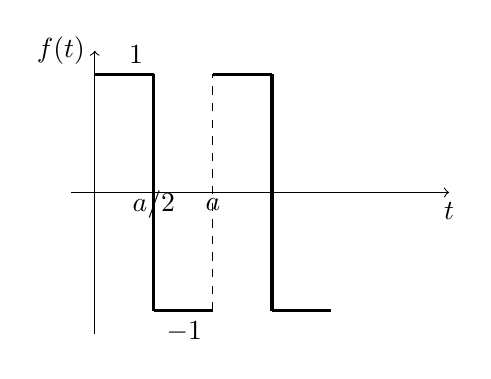
\begin{tikzpicture}[scale=1.5]
			\draw[->] (-0.2,0) -- (3,0) node[below] {$t$};
			\draw[->] (0,-1.2) -- (0,1.2) node[left] {$f(t)$};
			\draw[very thick] (0,1) -- (0.5,1) node[above left] {$1$};
			\draw[very thick] (0.5,1) -- (0.5,-1);
			\draw[very thick] (0.5,-1) -- (1,-1) node[below left] {$-1$};
			\draw[dashed] (1,-1) -- (1,1);
			\draw[very thick] (1,1) -- (1.5,1);
			\draw[very thick] (1.5,1) -- (1.5,-1);
			\draw[very thick] (1.5,-1) -- (2,-1);
			\node at (0.5, -0.1) {$a/2$};
			\node at (1, -0.1) {$a$};
		\end{tikzpicture}
	\end{center}
	\begin{align*}
		F(p) &= \frac{\int_0^a f(t) e^{-pt} dt}{1-e^{-pa}} \\
		\int_0^a f(t) e^{-pt} dt &= \int_0^{a/2} (1) e^{-pt} dt + \int_{a/2}^a (-1) e^{-pt} dt \\
		&= \left[-\frac{1}{p}e^{-pt}\right]_0^{a/2} - \left[-\frac{1}{p}e^{-pt}\right]_{a/2}^a \\
		&= -\frac{1}{p}(e^{-pa/2}-1) + \frac{1}{p}(e^{-pa}-e^{-pa/2}) = \frac{1}{p}(1 - 2e^{-pa/2} + e^{-pa}) = \frac{(1-e^{-pa/2})^2}{p} \\
		F(p) &= \frac{(1-e^{-pa/2})^2}{p(1-e^{-pa})} = \frac{(1-e^{-pa/2})^2}{p(1-e^{-pa/2})(1+e^{-pa/2})} = \frac{1-e^{-pa/2}}{p(1+e^{-pa/2})} \\
		&= \frac{e^{pa/4}-e^{-pa/4}}{p(e^{pa/4}+e^{-pa/4})} = \frac{2\sinh(pa/4)}{p(2\cosh(pa/4))} = \frac{1}{p}\tanh\left(\frac{pa}{4}\right)
	\end{align*}
	
	%====================================================================
	\section*{应用:求解偏微分方程}
	%====================================================================
	
	\subsection*{1. 弦振动方程 (Wave Equation)}
	方程为 $\frac{\partial^2 u}{\partial t^2} = a^2 \frac{\partial^2 u}{\partial x^2}$,其中 $a^2=T/\rho$。
	设初始条件为 $u(x,0) = f(x)$, $u_t(x,0)=g(x)$。对时间 $t$ 进行拉普拉斯变换:
	\begin{align*}
		& \mathcal{L}\left[\frac{\partial^2 u}{\partial t^2}\right] = a^2 \mathcal{L}\left[\frac{\partial^2 u}{\partial x^2}\right] \\
		& p^2 U(x,p) - p u(x,0) - u_t(x,0) = a^2 \frac{d^2 U(x,p)}{dx^2} \\
		& \frac{d^2 U}{dx^2} - \frac{p^2}{a^2}U = -\frac{p}{a^2}f(x) - \frac{1}{a^2}g(x)
	\end{align*}
	这是一个关于 $x$ 的二阶常微分方程。求解 $U(x,p)$ 后再进行拉普拉斯逆变换得到 $u(x,t)$。\\
	对于稳态振动解,可设 $u(x,t)=X(x)e^{i\omega t}$,代入原方程得到亥姆霍兹方程 (Helmholtz equation):
	$$ 
	\frac{d^2 X}{dx^2} + k^2 X = 0, \quad (k=\omega/a) 
	$$
	其通解为 $X(x) = A e^{ikx} + B e^{-ikx}$,代表了沿 x 轴正负方向传播的波。
	
	\subsection*{2. 输电线方程 (Telegrapher's Equation)}
	对于一段微元 $\Delta x$,电压和电流满足:
	\begin{align*}
		& \frac{\partial V}{\partial x} = -RI - L \frac{\partial I}{\partial t} \\
		& \frac{\partial I}{\partial x} = -GV - C \frac{\partial V}{\partial t}
	\end{align*}
	将两式联立消去 $I$,得到关于 $V$ 的电报方程:
	$$ 
	\frac{\partial^2 V}{\partial x^2} = LC \frac{\partial^2 V}{\partial t^2} + (RC+LG) \frac{\partial V}{\partial t} + GRV 
	$$
	\textbf{无损耗情况}: $R=0, G=0$。方程简化为波动方程 $\frac{\partial^2 V}{\partial x^2} = LC \frac{\partial^2 V}{\partial t^2}$。
	\textbf{正弦稳态分析}: 设 $V(x,t) = V(x)e^{i\omega t}$,$I(x,t) = I(x)e^{i\omega t}$。
	\begin{align*}
		& \frac{dV(x)}{dx} = -(R+i\omega L)I(x) = -Z I(x) \\
		& \frac{dI(x)}{dx} = -(G+i\omega C)V(x) = -Y V(x)
	\end{align*}
	其中 $Z, Y$ 分别为串联阻抗和并联导纳。再次微分可得:
	$$ 
	\frac{d^2 V(x)}{dx^2} = ZY \cdot V(x) = \gamma^2 V(x) 
	$$
	其中 $\gamma = \sqrt{ZY} = \sqrt{(R+i\omega L)(G+i\omega C)}$ 称为传播常数。
	$\gamma = \alpha + i\beta$,$\alpha$ 是衰减常数,$\beta$ 是相移常数。
	\textbf{无失真条件}: 为了让信号在传播过程中波形不发生改变,要求相速度 $v_p = \omega/\beta$ 与频率无关。这发生在 $\frac{RC}{LC} = \frac{LG}{LC}$,即 $\frac{R}{L} = \frac{G}{C}$ (Heaviside condition)。
	
	%====================================================================
	\section*{热传导方程}
	%====================================================================
	
	\subsection*{一维杆的热传导方程}
	考虑一维杆,长度为L,截面积为A。
	
	物理量:
	\begin{itemize}
		\item $u(x,t)$: $x$点在$t$时刻的温度
		\item $c$: 比热容
		\item $\rho$: 密度
		\item $Q$: 热量
	\end{itemize}
	
	\textbf{定律:} 单位时间内截面热流量
	$$ 
	Q = -kA \frac{\partial u}{\partial x} 
	$$
	其中$k$是热导率。
	
	考虑$[x, x+\Delta x]$一小段,在$\Delta t$时间内热量变化:
	$$ \Delta Q = Q_1 - Q_2 $$
	$$ Q_1 = -kA \frac{\partial u}{\partial x} \Big|_x \Delta t $$
	$$ Q_2 = -kA \frac{\partial u}{\partial x} \Big|_{x+\Delta x} \Delta t $$
	$$ \Delta Q = c \rho (A \Delta x) \Delta u = c \rho A \Delta x (u(t+\Delta t) - u(t)) $$
	($P=m/V$, $\Delta m = \rho A \Delta x$, 质量守恒)
	$$ \Rightarrow kA \Delta t \left( \frac{\partial u}{\partial x} \Big|_{x+\Delta x} - \frac{\partial u}{\partial x} \Big|_x \right) = c \rho A \Delta x \Delta u $$
	$$ \Rightarrow k \frac{\frac{\partial u}{\partial x} \Big|_{x+\Delta x} - \frac{\partial u}{\partial x} \Big|_x}{\Delta x} = c \rho \frac{\Delta u}{\Delta t} $$
	令$\Delta x, \Delta t \to 0$:
	$$ k \frac{\partial^2 u}{\partial x^2} = c \rho \frac{\partial u}{\partial t} $$
	$$ \frac{\partial u}{\partial t} = a^2 \frac{\partial^2 u}{\partial x^2} \quad (a^2 = \frac{k}{c\rho}) $$
	
	\textbf{热源情形:} 若有热源$f(x,t)$
	$$ 
	\frac{\partial u}{\partial t} = a^2 \frac{\partial^2 u}{\partial x^2} + f(x,t) 
	$$
	若热源由电流产生 $Q_{gen} = I^2 R \Delta t = j^2 \rho_e \delta \Delta x \Delta t$
	$$ Q_1 - Q_2 + Q_{gen} = \Delta Q $$
	$$ kA \Delta t \frac{\partial^2 u}{\partial x^2} \Delta x + j^2 \rho_e \delta \Delta x \Delta t = c \rho \delta \Delta x \Delta u $$
	$$ \Rightarrow \frac{\partial u}{\partial t} = a^2 \frac{\partial^2 u}{\partial x^2} + f $$
	$$ (c\rho \frac{\partial u}{\partial t} = k \frac{\partial^2 u}{\partial x^2} + F) $$
	
	\textbf{例:} 稳定状态 $\frac{\partial u}{\partial t}=0$
	$$ 
	a^2 \frac{\partial^2 u}{\partial x^2} + f = 0 \Rightarrow \frac{\partial^2 u}{\partial x^2} = 0 \quad (\text{若} f=0) 
	$$
	$$ u(x) = Ax + B $$
	
	%====================================================================
	\section*{电磁波方程}
	%====================================================================
	麦克斯韦方程组 ($\rho=0, j=0$ 真空中)
	$$ \nabla \cdot E = 0 $$
	$$ \nabla \cdot B = 0 $$
	$$ \nabla \times E = -\frac{\partial B}{\partial t} $$
	$$ \nabla \times B = \mu_0 \epsilon_0 \frac{\partial E}{\partial t} $$
	其中 $\epsilon_0 \mu_0 = 1/c^2$。
	
	\textbf{推导波动方程:}
	利用恒等式 $\nabla \times (\nabla \times A) = \nabla(\nabla \cdot A) - \Delta A$
	$$ \nabla \times (\nabla \times E) = \nabla(\nabla \cdot E) - \Delta E = -\Delta E $$
	$$ \nabla \times (-\frac{\partial B}{\partial t}) = -\frac{\partial}{\partial t}(\nabla \times B) = -\mu_0 \epsilon_0 \frac{\partial^2 E}{\partial t^2} $$
	$$ \Rightarrow \Delta E = \mu_0 \epsilon_0 \frac{\partial^2 E}{\partial t^2} $$
	$$ \frac{\partial^2 E}{\partial t^2} = c^2 \Delta E $$
	同理对$B$可得
	$$ \frac{\partial^2 B}{\partial t^2} = c^2 \Delta B $$
	
	\textbf{有源情况} ($\rho \neq 0, j \neq 0$)
	$$ \nabla \cdot E = \rho/\epsilon_0 $$
	$$ \nabla \cdot B = 0 $$
	$$ \nabla \times E = -\frac{\partial B}{\partial t} $$
	$$ \nabla \times B = \mu_0 j + \mu_0 \epsilon_0 \frac{\partial E}{\partial t} $$
	$$ \nabla \times (\nabla \times E) = \nabla(\rho/\epsilon_0) - \Delta E = -\frac{\partial}{\partial t}(\mu_0 j + \mu_0 \epsilon_0 \frac{\partial E}{\partial t}) $$
	$$ \Delta E - \mu_0 \epsilon_0 \frac{\partial^2 E}{\partial t^2} = \nabla(\rho/\epsilon_0) + \mu_0 \frac{\partial j}{\partial t} $$
	
	%====================================================================
	\section*{泊松方程}
	%====================================================================
	当$\rho \neq 0, j=0$ (静电场)
	$$ \Delta E = \nabla(\rho/\epsilon_0) $$
	引入电势$\phi$,$E = -\nabla\phi$
	$$ \Delta(-\nabla\phi) = -\nabla(\Delta\phi) = \nabla(\rho/\epsilon_0) $$
	$$ \Delta\phi = -\rho/\epsilon_0 $$
	此为泊松方程。
	无源情形 ($\rho=0$)
	$$ \Delta\phi = 0 $$
	此为拉普拉斯方程。
	
	%====================================================================
	\section*{二阶线性偏微分方程的分类}
	%====================================================================
	考虑方程:
	$$ 
	A \frac{\partial^2 u}{\partial x^2} + 2B \frac{\partial^2 u}{\partial x \partial y} + C \frac{\partial^2 u}{\partial y^2} + D \frac{\partial u}{\partial x} + E \frac{\partial u}{\partial y} + F u = G 
	$$
	其中$A, B, C, D, E, F, G$是$x, y$的函数。
	令 $\Delta = B^2 - AC$
	\begin{itemize}
		\item $\Delta > 0$: 双曲型 (e.g. 波动方程)
		\item $\Delta = 0$: 抛物型 (e.g. 热传导方程)
		\item $\Delta < 0$: 椭圆型 (e.g. 拉普拉斯方程)
	\end{itemize}
	这与二次曲线的分类是类似的。
	
	\textbf{坐标变换}
	令 $\xi = \xi(x,y), \eta = \eta(x,y)$
	$$ \frac{\partial u}{\partial x} = \frac{\partial u}{\partial \xi} \frac{\partial \xi}{\partial x} + \frac{\partial u}{\partial \eta} \frac{\partial \eta}{\partial x} $$
	$$ \frac{\partial u}{\partial y} = \frac{\partial u}{\partial \xi} \frac{\partial \xi}{\partial y} + \frac{\partial u}{\partial \eta} \frac{\partial \eta}{\partial y} $$
	$$ \frac{\partial^2 u}{\partial x^2} = \frac{\partial}{\partial x} (\frac{\partial u}{\partial x}) = \dots $$
	代入原方程,得到新的方程:
	$$ 
	a \frac{\partial^2 u}{\partial \xi^2} + 2b \frac{\partial^2 u}{\partial \xi \partial \eta} + c \frac{\partial^2 u}{\partial \eta^2} + \dots = G 
	$$
	其中
	$$ a = A(\frac{\partial \xi}{\partial x})^2 + 2B \frac{\partial \xi}{\partial x} \frac{\partial \xi}{\partial y} + C(\frac{\partial \xi}{\partial y})^2 $$
	$$ b = A \frac{\partial \xi}{\partial x} \frac{\partial \eta}{\partial x} + B (\frac{\partial \xi}{\partial x} \frac{\partial \eta}{\partial y} + \frac{\partial \xi}{\partial y} \frac{\partial \eta}{\partial x}) + C \frac{\partial \xi}{\partial y} \frac{\partial \eta}{\partial y} $$
	$$ c = A(\frac{\partial \eta}{\partial x})^2 + 2B \frac{\partial \eta}{\partial x} \frac{\partial \eta}{\partial y} + C(\frac{\partial \eta}{\partial y})^2 $$
	可以证明 $b^2 - ac = (B^2 - AC) (\frac{\partial \xi}{\partial x} \frac{\partial \eta}{\partial y} - \frac{\partial \xi}{\partial y} \frac{\partial \eta}{\partial x})^2$
	其中后面的行列式是坐标变换的雅可比行列式。
	
	%====================================================================
	\section*{化为标准型}
	%====================================================================
	目标是选择$\xi, \eta$使得$a,c$中至少一个为0。
	令 $a=0$
	$$ A(\frac{\partial \xi}{\partial x})^2 + 2B \frac{\partial \xi}{\partial x} \frac{\partial \xi}{\partial y} + C(\frac{\partial \xi}{\partial y})^2 = 0 $$
	$$ A \left(\frac{\partial \xi / \partial x}{\partial \xi / \partial y}\right)^2 + 2B \left(\frac{\partial \xi / \partial x}{\partial \xi / \partial y}\right) + C = 0 $$
	根据隐函数定理,沿 $\xi(x,y)=const$ 曲线,有 $\frac{dy}{dx} = - \frac{\partial \xi / \partial x}{\partial \xi / \partial y}$
	$$ A\left(\frac{dy}{dx}\right)^2 - 2B\left(\frac{dy}{dx}\right) + C = 0 $$
	解出 $\frac{dy}{dx}$
	$$ \frac{dy}{dx} = \frac{2B \pm \sqrt{4B^2 - 4AC}}{2A} = \frac{B \pm \sqrt{B^2 - AC}}{A} $$
	这就是特征方程。
	
	\paragraph{(1) $\Delta = B^2 - AC > 0$ (双曲型)}
	有两个不同的实根 $\frac{dy}{dx} = \lambda_1, \frac{dy}{dx} = \lambda_2$。
	解这两个常微分方程,得到两个特征线族 $\phi(x,y) = c_1, \psi(x,y)=c_2$。
	令 $\xi = \phi(x,y), \eta = \psi(x,y)$。
	这样 $a=0, c=0$。方程化为
	$$ 
	2b \frac{\partial^2 u}{\partial \xi \partial \eta} + \dots = 0 \Rightarrow \frac{\partial^2 u}{\partial \xi \partial \eta} = \dots \quad (\text{标准型I}) 
	$$
	若再做变换 $\xi' = \xi+\eta, \eta' = \xi-\eta$,则
	$$ 
	\frac{\partial^2 u}{\partial \xi'^2} - \frac{\partial^2 u}{\partial \eta'^2} = \dots \quad (\text{标准型II}) 
	$$
	
	\paragraph{(2) $\Delta = B^2 - AC = 0$ (抛物型)}
	只有一个实根 $\frac{dy}{dx} = \frac{B}{A}$。
	解得一个特征线族 $\phi(x,y)=c$。
	令 $\xi = \phi(x,y)$,则 $a=0$。
	$\eta$可以任取与$\xi$无关的函数,例如$\eta=x$。
	此时$b=0$, $c \neq 0$。方程化为
	$$ 
	c \frac{\partial^2 u}{\partial \eta^2} = \dots \Rightarrow \frac{\partial^2 u}{\partial \eta^2} = \dots \quad (\text{标准型}) 
	$$
	
	\paragraph{(3) $\Delta = B^2 - AC < 0$ (椭圆型)}
	特征方程的根是共轭复数。
	$$ \frac{dy}{dx} = \frac{B \pm i\sqrt{AC-B^2}}{A} $$
	解也是共轭的,$\phi(x,y) \pm i\psi(x,y) = const$。
	令 $\xi = \phi(x,y), \eta = \psi(x,y)$。
	可以证明 $a=c, b=0$。
	方程化为
	$$ 
	a\left(\frac{\partial^2 u}{\partial \xi^2} + \frac{\partial^2 u}{\partial \eta^2}\right) = \dots \Rightarrow \frac{\partial^2 u}{\partial \xi^2} + \frac{\partial^2 u}{\partial \eta^2} = \dots \quad (\text{标准型}) 
	$$
	
	\subsection*{再探标准型变换}
	\begin{itemize}
		\item[(b)] $\Delta = 0$: (应为 $u_{\eta\eta}=0$)
		取变换
		$$ \xi = x, \quad \eta = y - \frac{B}{A}x $$
		则
		$$ \frac{\partial^2 u}{\partial \xi^2} + \frac{\partial^2 u}{\partial \eta^2} = -\frac{1}{A^2}(\dots) $$
		(笔记此处似有误,应化为 $\frac{\partial^2 u}{\partial \eta^2} = \dots$)
		\item[(c)] $\Delta < 0$: $u_{xx} + u_{yy} = 0$.
		取变换
		$$ \xi = y - \frac{B}{A}x, \quad \eta = \frac{\sqrt{AC-B^2}}{A}x $$
		$$ \Rightarrow \frac{\partial^2 u}{\partial \xi^2} + \frac{\partial^2 u}{\partial \eta^2} = \dots $$
	\end{itemize}
	
	\textbf{总结特征线法:}
	从 $A(\frac{dy}{dx})^2 - 2B(\frac{dy}{dx}) + C = 0$ 出发
	\begin{enumerate}
		\item[(a)] $\Delta > 0$: 两条实特征线
		$$ \frac{dy}{dx} = \frac{B \pm \sqrt{B^2-AC}}{A} $$
		解出 $\phi_1(x,y)=c_1, \phi_2(x,y)=c_2$。
		令 $\xi = \phi_1, \eta = \phi_2$。得标准型:
		$$ \frac{\partial^2 u}{\partial \xi \partial \eta} = d \frac{\partial u}{\partial \xi} + e \frac{\partial u}{\partial \eta} + f u + g $$
		\item[(b)] $\Delta = 0$: 一条实特征线
		$$ \frac{dy}{dx} = \frac{B}{A} $$
		解出 $\phi(x,y)=c$。
		令 $\xi=\phi(x,y)$, $\eta$可任取(如$\eta=x$)。得标准型:
		$$ \frac{\partial^2 u}{\partial \eta^2} = d \frac{\partial u}{\partial \xi} + e \frac{\partial u}{\partial \eta} + f u + g $$
		\item[(c)] $\Delta < 0$: 无实特征线
		取 $\xi = y - \frac{B}{A}x, \eta = \frac{\sqrt{AC-B^2}}{A}x$。得标准型:
		$$ \frac{\partial^2 u}{\partial \xi^2} + \frac{\partial^2 u}{\partial \eta^2} = d \frac{\partial u}{\partial \xi} + e \frac{\partial u}{\partial \eta} + f u + g $$
	\end{enumerate}
	
	\subsection*{例子}
	\begin{enumerate}
		\item $u_{xx} - u_{t t} + a u_t + b u_x = 0$
		$A=1, B=0, C=-1$. $\Delta = 0 - (1)(-1) = 1 > 0$ (双曲型)
		特征方程: $(\frac{dt}{dx})^2 - 1 = 0 \Rightarrow \frac{dt}{dx} = \pm 1$
		特征线: $t-x=c_1, t+x=c_2$
		令 $\xi = x-t, \eta=x+t$.
		
		\item $u_{xx} - 2u_{xt} - u_t = 0$
		$A=1, B=-1, C=0$. $\Delta = (-1)^2 - 0 = 1 > 0$ (双曲型)
		特征方程: $(\frac{dt}{dx})^2 + 2(\frac{dt}{dx}) = 0 \Rightarrow \frac{dt}{dx}( \frac{dt}{dx}+2) = 0$
		$\frac{dt}{dx}=0 \Rightarrow t=c_1$.
		$\frac{dt}{dx}=-2 \Rightarrow t+2x=c_2$.
		令 $\xi = t, \eta=t+2x$.
		
		\item $u_{xx} - 4u_{xy} + 3u_{yy} + 8u_y + x = 0$
		$A=1, B=-2, C=3$. $\Delta = (-2)^2 - 1 \cdot 3 = 1 > 0$ (双曲型)
		
		\item $y u_{xx} + x u_{yy} = 0$
		$A=y, B=0, C=x$. $\Delta = -xy$.
		\begin{itemize}
			\item $xy>0$ (I, III象限): 椭圆型
			\item $xy<0$ (II, IV象限): 双曲型
			\item $x=0$ 或 $y=0$: 抛物型
		\end{itemize}
	\end{enumerate}
	
	%====================================================================
	\section*{定解问题}
	%====================================================================
	
	\subsection*{一维波动方程}
	$$ \begin{cases}
		\frac{\partial^2 u}{\partial t^2} = a^2 \frac{\partial^2 u}{\partial x^2} & 0 < x < L, t>0 \\
		u|_{x=0}=0, u|_{x=L}=0 & \text{(边界条件)} \\
		u|_{t=0}=\phi(x) & \text{(初始位移)} \\
		\frac{\partial u}{\partial t}|_{t=0}=\psi(x) & \text{(初始速度)}
	\end{cases} $$
	
	\textbf{叠加原理:}
	对于线性齐次方程 $L(u)=0$,若 $u_1, u_2$ 是解,则 $c_1 u_1 + c_2 u_2$ 也是解。
	对于 $L(u) = F$ (非齐次方程),其通解为 $u = u_p + u_h$,其中 $u_p$ 是一个特解,$u_h$ 是对应齐次方程的通解。
	此性质可用于分解问题。
	
	\subsection*{一维热传导方程}
	$$ \begin{cases}
		\frac{\partial u}{\partial t} = k \frac{\partial^2 u}{\partial x^2} & 0 < x < L, t>0 \\
		u(0,t)=0, u(L,t)=0 & (t>0) \\
		u(x,0)=f(x) & (0 \le x \le L)
	\end{cases} $$
	这是一个定解问题。
	
	\textbf{例1:稳态解}
	如果边界条件不为零,如 $u(0,t)=T_1, u(L,t)=T_2$。
	稳态解 $u_E(x)$ 满足
	$$ \frac{d^2 u_E}{d x^2} = 0 \Rightarrow u_E(x) = c_1 x + c_2 $$
	代入边界条件
	$$ u_E(0)=T_1 \Rightarrow c_2=T_1 $$
	$$ u_E(L)=T_2 \Rightarrow c_1 L + T_1 = T_2 \Rightarrow c_1 = \frac{T_2-T_1}{L} $$
	所以
	$$ u_E(x) = \frac{T_2-T_1}{L}x + T_1 $$
	令 $u(x,t) = v(x,t) + u_E(x)$,则$v(x,t)$满足齐次边界条件。
	
	\section*{分离变量法 (Separation of Variables Method)}
	\subsection*{弦振动 (String Vibration)}
	
	\noindent The governing partial differential equation (PDE):
	$$ \frac{\partial^2 u}{\partial t^2} = a^2 \frac{\partial^2 u}{\partial x^2} $$
	Initial conditions:
	$$ u|_{t=0} = \phi(x) $$
	$$ \frac{\partial u}{\partial t}\bigg|_{t=0} = \psi(x) $$
	Boundary conditions (fixed ends):
	$$ u|_{x=0} = 0, \quad u|_{x=L} = 0 $$
	Goal: Find the solution $u(x,t)$.
	
	\subsection*{推导 (Derivation)}
	Assume the solution can be written as a product of functions of a single variable:
	$$ u(x,t) = X(x)T(t) $$
	Substitute into the PDE:
	$$ X(x)T''(t) = a^2 X''(x)T(t) $$
	Rearrange the terms to separate variables:
	$$ \frac{X''(x)}{X(x)} = \frac{T''(t)}{a^2 T(t)} $$
	Since the left side depends only on $x$ and the right side only on $t$, both must be equal to a constant. Let's call this constant $-\lambda$.
	$$ \frac{d}{dx}\left[\frac{X''(x)}{X(x)}\right] = 0 $$
	$$ \frac{d}{dt}\left[\frac{T''(t)}{a^2 T(t)}\right] = 0 $$
	This gives two ordinary differential equations (ODEs):
	$$ X''(x) + \lambda X(x) = 0 $$
	$$ T''(t) + \lambda a^2 T(t) = 0 $$
	The boundary conditions for $u(x,t)$ translate to conditions for $X(x)$, since $T(t) \not\equiv 0$ for a non-trivial solution:
	$$ u(0,t) = X(0)T(t) = 0 \implies X(0) = 0 $$
	$$ u(L,t) = X(L)T(t) = 0 \implies X(L) = 0 $$
	
	\subsection*{求解本征值问题 (Solving the Eigenvalue Problem for X(x))}
	We analyze the possible values of the separation constant $\lambda$.
	
	\paragraph{Case 1: $\lambda = 0$}
	The equation for $X(x)$ is $X''(x) = 0$.
	The general solution is:
	$$ X(x) = Ax + B $$
	Applying the boundary conditions:
	$$ X(0) = B = 0 $$
	$$ X(L) = AL + B = 0 \implies A = 0 $$
	This gives $X(x) = 0$, which leads to the trivial solution $u(x,t) = 0$.
	
	\paragraph{Case 2: $\lambda < 0$}
	Let $\lambda = -k^2$ where $k > 0$. The equation is $X''(x) - k^2 X(x) = 0$.
	The general solution is:
	$$ X(x) = A \cosh(kx) + B \sinh(kx) $$
	Applying the boundary conditions:
	$$ X(0) = A \cosh(0) + B \sinh(0) = A = 0 $$
	$$ X(L) = B \sinh(kL) = 0 $$
	Since $k>0$ and $L>0$, $\sinh(kL) \neq 0$, so $B=0$.
	This again leads to the trivial solution $X(x) = 0$.
	
	\paragraph{Case 3: $\lambda > 0$}
	Let $\lambda = k^2$ where $k > 0$. The equation is $X''(x) + k^2 X(x) = 0$.
	The general solution is:
	$$ X(x) = A \cos(kx) + B \sin(kx) $$
	Applying the boundary conditions:
	$$ X(0) = A \cos(0) + B \sin(0) = A = 0 $$
	So,
	$$ X(x) = B \sin(kx) $$
	$$ X(L) = B \sin(kL) = 0 $$
	For a non-trivial solution, we must have $B \neq 0$, which implies:
	$$ \sin(kL) = 0 $$
	This means $kL = n\pi$ for $n = 1, 2, 3, \dots$.
	The possible values for $k$ are:
	$$ k_n = \frac{n\pi}{L} $$
	These lead to the eigenvalues (本征值):
	$$ \lambda_n = k_n^2 = \left(\frac{n\pi}{L}\right)^2 $$
	The corresponding eigenfunctions (本征函数) are:
	$$ X_n(x) = B_n \sin\left(\frac{n\pi x}{L}\right) $$
	
	\subsection*{求解 T(t) 并叠加 (Solving for T(t) and Superposition)}
	Now we solve for $T(t)$ using the found eigenvalues $\lambda_n$:
	$$ T_n''(t) + \lambda_n a^2 T_n(t) = 0 $$
	$$ T_n''(t) + \left(\frac{n\pi a}{L}\right)^2 T_n(t) = 0 $$
	The general solution for $T_n(t)$ is:
	$$ T_n(t) = C_n \cos\left(\frac{n\pi a t}{L}\right) + D_n \sin\left(\frac{n\pi a t}{L}\right) $$
	The solution for each mode $n$ is $u_n(x,t) = X_n(x) T_n(t)$. We absorb the constant $B_n$ into $C_n$ and $D_n$.
	$$ u_n(x,t) = \left(C_n \cos\left(\frac{n\pi a t}{L}\right) + D_n \sin\left(\frac{n\pi a t}{L}\right)\right) \sin\left(\frac{n\pi x}{L}\right) $$
	By the superposition principle (叠加原理), the general solution is the sum of all possible solutions:
	$$ u(x,t) = \sum_{n=1}^{\infty} u_n(x,t) $$
	$$ u(x,t) = \sum_{n=1}^{\infty} \left(C_n \cos\left(\frac{n\pi a t}{L}\right) + D_n \sin\left(\frac{n\pi a t}{L}\right)\right) \sin\left(\frac{n\pi x}{L}\right) $$
	
	\subsection*{利用初始条件 (Using Initial Conditions)}
	We determine the coefficients $C_n$ and $D_n$ using the initial conditions.
	At $t=0$:
	$$ u(x,0) = \phi(x) = \sum_{n=1}^{\infty} C_n \sin\left(\frac{n\pi x}{L}\right) $$
	This is a Fourier sine series for $\phi(x)$. The coefficients $C_n$ are given by:
	$$ C_n = \frac{2}{L} \int_0^L \phi(x) \sin\left(\frac{n\pi x}{L}\right) dx $$
	Next, we find the derivative with respect to $t$:
	$$ \frac{\partial u}{\partial t} = \sum_{n=1}^{\infty} \left(-C_n \frac{n\pi a}{L} \sin\left(\frac{n\pi a t}{L}\right) + D_n \frac{n\pi a}{L} \cos\left(\frac{n\pi a t}{L}\right)\right) \sin\left(\frac{n\pi x}{L}\right) $$
	At $t=0$:
	$$ \frac{\partial u}{\partial t}\bigg|_{t=0} = \psi(x) = \sum_{n=1}^{\infty} D_n \frac{n\pi a}{L} \sin\left(\frac{n\pi x}{L}\right) $$
	This is a Fourier sine series for $\psi(x)$. The coefficients are given by:
	$$ D_n \frac{n\pi a}{L} = \frac{2}{L} \int_0^L \psi(x) \sin\left(\frac{n\pi x}{L}\right) dx $$
	$$ D_n = \frac{2}{n\pi a} \int_0^L \psi(x) \sin\left(\frac{n\pi x}{L}\right) dx $$
	
	\subsection*{分离变量法总结 (Summary of Separation of Variables)}
	\begin{enumerate}
		\item \textbf{分离变量:} 设定 $u=TX$ (Let $u=TX$)
		\item \textbf{定解:} 代入得 $X(x), T(t)$ 常微分方程 (Substitute to get ODEs for $X(x), T(t)$)
		\item \textbf{边界条件:} 求解 $X(x)$, 边界条件 (齐次) $\implies$ 本征值 $\lambda_n$ 与本征函数 $X_n(x)$ (Solve for $X(x)$ using homogeneous boundary conditions to get eigenvalues $\lambda_n$ and eigenfunctions $X_n(x)$)
		\item \textbf{齐次:} 代入 $\lambda_n \to T_n(t)$ (Substitute $\lambda_n$ to find $T_n(t)$)
		\item \textbf{叠加原理:} $u(x,t) = \sum u_n(x,t)$ (Superposition principle)
	\end{enumerate}
	
	\section*{基本解问题 (Examples of Fundamental Solutions)}
	\subsection*{例1 (Example 1: Plucked String)}
	Problem:
	$$ \frac{\partial^2 u}{\partial t^2} = a^2 \frac{\partial^2 u}{\partial x^2} $$
	$$ u(x,0) = \phi(x) = \begin{cases} \frac{3}{2}x & 0 \le x \le 2/5 \\ 3(1-x) & 2/5 \le x \le 1 \end{cases} \quad (\text{with } L=1) $$
	$$ \frac{\partial u}{\partial t}\bigg|_{t=0} = \psi(x) = 0 $$
	$$ u(0,t) = 0, \quad u(1,t) = 0 $$
	Since $\psi(x)=0$, we have $D_n=0$ for all $n$.
	We calculate $C_n$:
	$$ C_n = \frac{2}{1} \int_0^1 \phi(x) \sin(n\pi x) dx $$
	$$ C_n = 2 \left[ \int_0^{2/5} \frac{3}{2}x \sin(n\pi x) dx + \int_{2/5}^1 3(1-x) \sin(n\pi x) dx \right] $$
	After integration (result from notes):
	$$ C_n = \frac{9}{5n^2\pi^2} \sin\left(\frac{2n\pi}{5}\right) $$
	The final solution is:
	$$ u(x,t) = \sum_{n=1}^{\infty} \frac{9}{5n^2\pi^2} \sin\left(\frac{2n\pi}{5}\right) \cos(n\pi at) \sin(n\pi x) $$
	
	\subsection*{例2 (Example 2: Struck String)}
	Problem:
	$$ \frac{\partial^2 u}{\partial t^2} = a^2 \frac{\partial^2 u}{\partial x^2} $$
	$$ u(x,0) = \phi(x) = 0 $$
	$$ \frac{\partial u}{\partial t}\bigg|_{t=0} = \psi(x) = \frac{K}{\rho}\delta(x-c) \quad (\text{impulse at } x=c) $$
	$$ u(0,t) = 0, \quad u(L,t) = 0 $$
	Since $\phi(x)=0$, we have $C_n = 0$ for all $n$.
	We calculate $D_n$:
	$$ D_n = \frac{2}{n\pi a} \int_0^L \psi(x) \sin\left(\frac{n\pi x}{L}\right) dx $$
	$$ D_n = \frac{2}{n\pi a} \int_0^L \frac{K}{\rho} \delta(x-c) \sin\left(\frac{n\pi x}{L}\right) dx $$
	Using the sifting property of the Dirac delta function:
	$$ D_n = \frac{2K}{n\pi a \rho} \sin\left(\frac{n\pi c}{L}\right) $$
	The final solution is:
	$$ u(x,t) = \sum_{n=1}^{\infty} \frac{2K}{n\pi a \rho} \sin\left(\frac{n\pi c}{L}\right) \sin\left(\frac{n\pi a t}{L}\right) \sin\left(\frac{n\pi x}{L}\right) $$
	
	\section*{物理解释 (Physical Interpretation)}
	The solution for a single mode can be written in phase-amplitude form:
	$$ u_n(x,t) = N_n \sin(\omega_n t + \theta_n) \sin\left(\frac{n\pi x}{L}\right) $$
	where the angular frequency is $\omega_n = \frac{n\pi a}{L}$.
	The amplitude $N_n$ and phase $\theta_n$ are given by:
	$$ N_n = \sqrt{C_n^2+D_n^2} $$
	$$ \tan\theta_n = \frac{C_n}{D_n} $$
	An alternative form from the notes is:
	$$ u_n(x,t) = A_n(t) \sin\left(\frac{n\pi x}{L}\right) $$
	$$ u_n(t) = B_n(x_0) \sin(\omega_n t + \theta_n) $$
	
	\subsection*{驻波 (Standing Waves)}
	The solution $u_n(x,t)$ represents a standing wave.
	\begin{itemize}
		\item \textbf{节点 (Nodes):} Points that do not move. Occur when $\sin(\frac{n\pi x}{L}) = 0$.
		$$ \frac{n\pi x}{L} = m\pi, \quad m = 0, 1, \dots, n $$
		$$ x_m = \frac{m}{n}L $$
		\item \textbf{波腹 (Antinodes):} Points of maximum amplitude ($x_0$).
	\end{itemize}
	
	\subsection*{单模振动 (Single-mode Oscillation)}
	A single eigenfunction corresponds to a single mode of vibration.
	$$ E \sim \sin\left(\frac{n\pi x}{L}\right) $$
	
	\subsection*{与量子力学类比 (Analogy to Quantum Mechanics)}
	The spatial part of the wave solution is analogous to the wave function for a particle in a 1D infinite potential well.
	$$ \Psi \sim \sin\left(\frac{n\pi x}{L}\right) $$
	The time-dependent Schrödinger equation:
	$$ i\hbar \frac{\partial \Psi}{\partial t} = -\frac{\hbar^2}{2m} \nabla^2 \Psi + U(x)\Psi $$
	
	\section*{其他边界条件 (Other Boundary Conditions)}
	\begin{enumerate}
		\item \textbf{两端固定 (Fixed-Fixed):} $u(0,t)=0$, $u(L,t)=0$.
		\item \textbf{一端固定, 一端自由 (Fixed-Free):} $u(0,t)=0$, $\frac{\partial u}{\partial x}\bigg|_{x=L}=0$.
		\item \textbf{两端自由 (Free-Free):} $\frac{\partial u}{\partial x}\bigg|_{x=0}=0$, $\frac{\partial u}{\partial x}\bigg|_{x=L}=0$.
		\item \textbf{辐射边界条件 (Radiation Boundary Condition):} $-k\frac{\partial u}{\partial x}\bigg|_{x=L} = H(u(L,t) - u_0)$.
	\end{enumerate}
	
	\section*{有阻尼波动方程与电报方程 (Damped Wave and Telegrapher's Equation)}
	
	\subsection*{例: 电报方程 (Example: Telegrapher's Equation)}
	The general form of the Telegrapher's equation is:
	$$ \frac{\partial^2 u}{\partial t^2} - a^2 \frac{\partial^2 u}{\partial x^2} + 2b \frac{\partial u}{\partial t} + c u = 0 $$
	With initial conditions:
	$$ u|_{t=0} = \phi(x) $$
	$$ \frac{\partial u}{\partial t}\bigg|_{t=0} = \psi(x) $$
	And boundary conditions ($b, c > 0$):
	$$ u|_{x=0} = 0, \quad u|_{x=L} = 0 $$
	Using separation of variables, $u(x,t) = X(x)T(t)$, we get:
	$$ X''(x) + \lambda X(x) = 0 $$
	$$ X(0) = 0, \quad X(L) = 0 $$
	and
	$$ T''(t) + 2b T'(t) + (\lambda a^2 + c) T(t) = 0 $$
	The solution for $X(x)$ is the same as for the standard wave equation:
	$$ \lambda_n = \left(\frac{n\pi}{L}\right)^2 $$
	$$ X_n(x) = B_n \sin\left(\frac{n\pi x}{L}\right) $$
	The solution for $T(t)$ is that of a damped harmonic oscillator. For the underdamped case, the solution has the form:
	$$ u(x,t) = e^{-bt} \sum_{n=1}^{\infty} \left(C_n \cos(q_n t) + D_n \sin(q_n t)\right) \sin\left(\frac{n\pi x}{L}\right) $$
	where the new frequency $q_n$ is:
	$$ q_n = \sqrt{\left|\left(\frac{n\pi a}{L}\right)^2 + c - b^2\right|} $$
	The coefficients $C_n, D_n$ are determined by the initial conditions.
	
	\subsection*{例: 有阻尼波动方程 (Example: Damped Wave Equation)}
	This is a special case of the Telegrapher's equation where $c=0$.
	$$ \frac{\partial^2 u}{\partial t^2} - a^2 \frac{\partial^2 u}{\partial x^2} + 2b \frac{\partial u}{\partial t} = 0 $$
	The equation for $T(t)$ becomes:
	$$ T_n''(t) + 2b T_n'(t) + \lambda_n a^2 T_n(t) = 0 $$
	The characteristic equation is $r^2 + 2br + (\frac{n\pi a}{L})^2 = 0$. The behavior depends on the discriminant. Let $q_n = \sqrt{\left| (\frac{n\pi a}{L})^2 - b^2 \right|}$.
	
	The general solution for $T_n(t)$ can be one of three cases for each mode $n$:
	\begin{enumerate}
		\item \textbf{Underdamped} ($\frac{n\pi a}{L} > b$):
		$$ T_n(t) = e^{-bt} \left(C_n \cos(q_n t) + D_n \sin(q_n t)\right) $$
		\item \textbf{Critically Damped} ($\frac{n\pi a}{L} = b$):
		$$ T_n(t) = e^{-bt} (C_n + D_n t) $$
		\item \textbf{Overdamped} ($\frac{n\pi a}{L} < b$):
		$$ T_n(t) = e^{-bt} \left(C_n \cosh(q_n t) + D_n \sinh(q_n t)\right) $$
	\end{enumerate}
	Let's assume the underdamped case holds for all modes of interest ($\frac{bL}{\pi a} < 1$). The total solution is:
	$$ u(x,t) = \sum_{n=1}^{\infty} e^{-bt} \left(C_n \cos(q_n t) + D_n \sin(q_n t)\right) \sin\left(\frac{n\pi x}{L}\right) $$
	To find the coefficients from $u(x,0) = \phi(x)$ and $u_t(x,0)=\psi(x)$:
	$$ \phi(x) = \sum_{n=1}^{\infty} C_n \sin\left(\frac{n\pi x}{L}\right) $$
	$$ \implies C_n = \frac{2}{L} \int_0^L \phi(x) \sin\left(\frac{n\pi x}{L}\right) dx $$
	$$ \psi(x) = \sum_{n=1}^{\infty} (-b C_n + q_n D_n) \sin\left(\frac{n\pi x}{L}\right) $$
	$$ \implies -b C_n + q_n D_n = \frac{2}{L} \int_0^L \psi(x) \sin\left(\frac{n\pi x}{L}\right) dx $$
	$$ \implies D_n = \frac{b}{q_n} C_n + \frac{2}{q_n L} \int_0^L \psi(x) \sin\left(\frac{n\pi x}{L}\right) dx $$
	If the initial velocity is zero, $\psi(x)=0$, then $D_n = \frac{b}{q_n}C_n$.
	
	\newpage
	\section*{热传导方程 (Heat Equation)}
	\subsection*{例: 傅里叶热棒 (Example: Fourier Heat Rod)}
	The problem describes the temperature $u(x,t)$ in a rod with insulated ends.
	$$ \frac{\partial u}{\partial t} = a^2 \frac{\partial^2 u}{\partial x^2} $$
	Initial condition:
	$$ u(t=0) = \phi(x) $$
	Boundary conditions (insulated ends):
	$$ \frac{\partial u}{\partial x}\bigg|_{x=0} = 0, \quad \frac{\partial u}{\partial x}\bigg|_{x=L} = 0 $$
	Separating variables $u(x,t) = X(x)T(t)$ yields:
	$$ X''(x) + \lambda X(x) = 0, \quad \text{with } X'(0)=0, X'(L)=0 $$
	$$ T'(t) + \lambda a^2 T(t) = 0 $$
	Solving the eigenvalue problem for $X(x)$:
	\begin{itemize}
		\item Case $\lambda=0$: $X''(x)=0 \implies X(x) = Ax+B$. $X'(0)=A=0$. $X'(L)=A=0$. So $X_0(x) = B_0$ (a constant) is an eigenfunction.
		\item Case $\lambda < 0$: Trivial solution $X(x)=0$.
		\item Case $\lambda > 0$ ($\lambda=k^2$): $X(x) = A\cos(kx)+B\sin(kx)$. $X'(0) = B k = 0 \implies B=0$. $X'(L) = -A k \sin(kL) = 0 \implies \sin(kL)=0$. Thus $kL=n\pi$ for $n=1,2,3,\dots$.
	\end{itemize}
	The eigenvalues are $\lambda_n = (\frac{n\pi}{L})^2$ for $n=0, 1, 2, \dots$.
	The eigenfunctions are $X_n(x) = A_n \cos(\frac{n\pi x}{L})$.
	Solving for $T(t)$:
	For $n>0$: $T_n'(t) + (\frac{n\pi a}{L})^2 T_n(t) = 0 \implies T_n(t) = C_n e^{-(\frac{n\pi a}{L})^2 t}$.
	For $n=0$ ($\lambda_0=0$): $T_0'(t)=0 \implies T_0(t) = C_0$.
	The general solution is by superposition:
	$$ u(x,t) = C_0 + \sum_{n=1}^{\infty} C_n \exp\left[-\left(\frac{n\pi a}{L}\right)^2 t\right] \cos\left(\frac{n\pi x}{L}\right) $$
	Using the initial condition $u(x,0)=\phi(x)$:
	$$ \phi(x) = C_0 + \sum_{n=1}^{\infty} C_n \cos\left(\frac{n\pi x}{L}\right) $$
	This is a Fourier cosine series. The coefficients are:
	$$ C_0 = \frac{1}{L} \int_0^L \phi(x) dx $$
	$$ C_n = \frac{2}{L} \int_0^L \phi(x) \cos\left(\frac{n\pi x}{L}\right) dx $$
	
	\newpage
	\section*{波动方程更多示例 (Further Examples for the Wave Equation)}
	\subsection*{例: 自由-固定端 (Example: Free-Fixed End)}
	The note appears to solve for a rod with a free end at $x=0$ and a fixed end at $x=L$.
	$$ \frac{\partial^2 u}{\partial t^2} = a^2 \frac{\partial^2 u}{\partial x^2} $$
	$$ \frac{\partial u}{\partial x}\bigg|_{x=0}=0, \quad u|_{x=L}=0 $$
	Separation of variables leads to $X''(x)+\lambda X(x)=0$ with $X'(0)=0, X(L)=0$.
	Let $\lambda=k^2$. $X(x)=A\cos(kx)+B\sin(kx)$.
	$$ X'(0) = B k = 0 \implies B=0 $$
	$$ X(L) = A\cos(kL) = 0 \implies kL = \frac{(2n+1)\pi}{2}, \quad n=0, 1, 2, \dots $$
	The eigenvalues and eigenfunctions are:
	$$ \lambda_n = \left(\frac{(2n+1)\pi}{2L}\right)^2 $$
	$$ X_n(x) = A_n \cos\left(\frac{(2n+1)\pi x}{2L}\right) $$
	The general solution is:
	$$ u(x,t) = \sum_{n=0}^{\infty} \left(C_n \cos\left(\frac{(2n+1)\pi a t}{2L}\right) + D_n \sin\left(\frac{(2n+1)\pi a t}{2L}\right)\right) \cos\left(\frac{(2n+1)\pi x}{2L}\right) $$
	Coefficients are found from initial conditions $\phi(x)$ and $\psi(x)$:
	$$ C_n = \frac{2}{L} \int_0^L \phi(x) \cos\left(\frac{(2n+1)\pi x}{2L}\right) dx $$
	$$ D_n = \frac{2}{L} \frac{2L}{(2n+1)\pi a} \int_0^L \psi(x) \cos\left(\frac{(2n+1)\pi x}{2L}\right) dx $$
	\paragraph{Specific Case:} If $u(x,0) = \cos(\frac{\pi x}{2L})$ and $u_t(x,0)=0$.
	This corresponds to the $n=0$ mode.
	$$ D_n = 0 \text{ for all } n $$
	$$ C_n = \frac{2}{L} \int_0^L \cos\left(\frac{\pi x}{2L}\right) \cos\left(\frac{(2n+1)\pi x}{2L}\right) dx $$
	By orthogonality, this integral is non-zero only for $n=0$.
	$$ C_0 = \frac{2}{L} \int_0^L \cos^2\left(\frac{\pi x}{2L}\right) dx = \frac{2}{L} \cdot \frac{L}{2} = 1 $$
	All other $C_n=0$. The solution is:
	$$ u(x,t) = \cos\left(\frac{\pi a t}{2L}\right) \cos\left(\frac{\pi x}{2L}\right) $$
	
	\subsection*{例: 固定-自由端 (Example: Fixed-Free End)}
	Another example shows fixed-free boundary conditions: $u(0,t)=0, u_x(L,t)=0$.
	Eigenfunctions: $\sin(\frac{(2n+1)\pi x}{2L})$.
	Initial conditions: $u(x,0)=E$ (a constant), $u_t(x,0)=0$.
	Then $D_n=0$ for all $n$.
	$$ C_n = \frac{2}{L} \int_0^L E \sin\left(\frac{(2n+1)\pi x}{2L}\right) dx $$
	$$ C_n = \frac{2E}{L} \left[-\frac{2L}{(2n+1)\pi} \cos\left(\frac{(2n+1)\pi x}{2L}\right) \right]_0^L $$
	$$ C_n = -\frac{4E}{(2n+1)\pi} (\cos(\frac{(2n+1)\pi}{2}) - \cos(0)) = \frac{4E}{(2n+1)\pi} $$
	The solution is:
	$$ u(x,t) = \frac{4E}{\pi} \sum_{n=0}^{\infty} \frac{1}{2n+1} \cos\left(\frac{(2n+1)\pi a t}{2L}\right) \sin\left(\frac{(2n+1)\pi x}{2L}\right) $$
	总结 (Summary)
	$$
	X''(x) + \lambda X(x) = 0
	$$
	$$
	u|_{x=0} = u|_{x=L} = 0 \quad \Rightarrow \quad \lambda_n = (\frac{n\pi}{L})^2, \quad X_n(x) = B_n \sin(\frac{n\pi x}{L})
	$$
	$$
	\frac{\partial u}{\partial x}|_{x=0} = \frac{\partial u}{\partial x}|_{x=L} = 0 \quad \Rightarrow \quad \lambda_n = (\frac{n\pi}{L})^2, \quad X_n(x) = A_n \cos(\frac{n\pi x}{L})
	$$
	$$
	u|_{x=0} = \frac{\partial u}{\partial x}|_{x=L} = 0 \quad \Rightarrow \quad \lambda_n = (\frac{(2n+1)\pi}{2L})^2, \quad X_n(x) = A_n \cos(\frac{(2n+1)\pi x}{2L})
	$$
	
	二维波动方程 (2D Wave Equation)
	$$
	\frac{\partial^2 u}{\partial t^2} = c^2 (\frac{\partial^2 u}{\partial x^2} + \frac{\partial^2 u}{\partial y^2})
	$$
	$$
	\begin{cases}
		u|_{t=0} = \phi(x,y) \\
		u_t|_{t=0} = \psi(x,y) \\
		u|_{x=0} = u|_{x=a} = 0 \quad 0 \le y \le b \\
		u|_{y=0} = u|_{y=b} = 0 \quad 0 \le x \le a
	\end{cases}
	$$
	令 (Let)
	$$
	u(x,y,t) = V(x,y)T(t)
	$$
	$$
	\Rightarrow \frac{T''}{c^2 T} = \frac{1}{V}(\frac{\partial^2 V}{\partial x^2} + \frac{\partial^2 V}{\partial y^2}) = -\lambda
	$$
	$$
	\Rightarrow \frac{\partial^2 V}{\partial x^2} + \frac{\partial^2 V}{\partial y^2} + \lambda V = 0
	$$
	$$
	T'' + \lambda c^2 T = 0
	$$
	再令 (Let again)
	$$
	V(x,y) = X(x)Y(y)
	$$
	$$
	\Rightarrow \frac{X''}{X} = -\frac{Y''+\lambda Y}{Y} = -\mu
	$$
	$$
	\Rightarrow \begin{cases}
		X''+\mu X=0 \\
		X(0)=X(a)=0
	\end{cases}
	$$
	$$
	\begin{cases}
		Y''+\nu Y=0, \quad \nu = \lambda - \mu \\
		Y(0)=Y(b)=0
	\end{cases}
	$$
	解得 (Solution is)
	$$
	\mu_m = (\frac{m\pi}{a})^2, \quad X_m(x) = \sin(\frac{m\pi x}{a})
	$$
	$$
	\nu_n = (\frac{n\pi}{b})^2, \quad Y_n(y) = \sin(\frac{n\pi y}{b})
	$$
	到 (Thus)
	$$
	\lambda_{mn} = (\frac{m\pi}{a})^2 + (\frac{n\pi}{b})^2
	$$
	$$
	V_{mn}(x,y) = \sin(\frac{m\pi x}{a}) \sin(\frac{n\pi y}{b})
	$$
	代入 (Substitute into T)
	$$
	T_{mn}(t) = C_{mn} \cos(\omega_{mn} t) + D_{mn} \sin(\omega_{mn} t)
	$$
	$$
	\omega_{mn} = c \sqrt{\lambda_{mn}} = c\pi \sqrt{(\frac{m}{a})^2 + (\frac{n}{b})^2}
	$$
	基频 (Fundamental frequency)
	$$
	\omega_{11} = c\pi \sqrt{\frac{1}{a^2} + \frac{1}{b^2}}
	$$
	叠加 (Superposition)
	$$
	u(x,y,t) = \sum_{m=1}^{\infty} \sum_{n=1}^{\infty} u_{mn}(x,y,t) = \sum_{m=1}^{\infty} \sum_{n=1}^{\infty} (C_{mn} \cos(\omega_{mn} t) + D_{mn} \sin(\omega_{mn} t)) \sin(\frac{m\pi x}{a})\sin(\frac{n\pi y}{b})
	$$
	$$
	\phi(x,y) = \sum_{m=1}^{\infty} \sum_{n=1}^{\infty} C_{mn} \sin(\frac{m\pi x}{a})\sin(\frac{n\pi y}{b})
	$$
	$$
	\psi(x,y) = \sum_{m=1}^{\infty} \sum_{n=1}^{\infty} \omega_{mn} D_{mn} \sin(\frac{m\pi x}{a})\sin(\frac{n\pi y}{b})
	$$
	正交性 (Orthogonality)
	$$
	\int_0^a \int_0^b V_{mn}(x,y) V_{m'n'}(x,y) dx dy = (\int_0^a \sin(\frac{m\pi x}{a})\sin(\frac{m'\pi x}{a}) dx)(\int_0^b \sin(\frac{n\pi y}{b})\sin(\frac{n'\pi y}{b}) dy)
	$$
	$$
	= \frac{ab}{4} \delta_{mm'} \delta_{nn'}
	$$
	得 (We get)
	$$
	C_{mn} = \frac{4}{ab} \int_0^a \int_0^b \phi(x,y) \sin(\frac{m\pi x}{a})\sin(\frac{n\pi y}{b}) dx dy
	$$
	$$
	D_{mn} = \frac{4}{ab \omega_{mn}} \int_0^a \int_0^b \psi(x,y) \sin(\frac{m\pi x}{a})\sin(\frac{n\pi y}{b}) dx dy
	$$
	特征函数集 (Set of eigenfunctions)
	$$
	\{ \sin(\frac{m\pi x}{a}) \sin(\frac{n\pi y}{b}) \}
	$$
	例 (Example)
	$$
	a=b=1, \quad c = \frac{1}{\pi}
	$$
	$$
	\phi = x(1-x)y(1-y)
	$$
	$$
	\psi = 0 \quad \Rightarrow \quad D_{mn}=0
	$$
	$$
	C_{mn} = 4 \int_0^1 \int_0^1 x(1-x)y(1-y) \sin(m\pi x)\sin(n\pi y) dx dy
	$$
	$$
	= 4 [\int_0^1 x(1-x) \sin(m\pi x) dx] [\int_0^1 y(1-y) \sin(n\pi y) dy]
	$$
	$$
	\int_0^1 x(1-x) \sin(m\pi x) dx = \frac{2(1-(-1)^m)}{m^3\pi^3}
	$$
	$$
	C_{mn} = 4 \frac{2(1-(-1)^m)}{m^3\pi^3} \frac{2(1-(-1)^n)}{n^3\pi^3} = \frac{16(1-(-1)^m)(1-(-1)^n)}{m^3 n^3 \pi^6}
	$$
	解 (Solution)
	$$
	u = \sum_{m,n=1,3,5,...}^{\infty} \frac{64}{\pi^6 m^3 n^3} \cos(\sqrt{m^2+n^2}t) \sin(m\pi x)\sin(n\pi y)
	$$
	
	二维热传导方程 (2D Heat Equation)
	$$
	\frac{\partial u}{\partial t} = c^2 (\frac{\partial^2 u}{\partial x^2} + \frac{\partial^2 u}{\partial y^2})
	$$
	$$
	u|_{t=0} = \phi(x,y)
	$$
	$$
	u|_{x=0}=u|_{x=a}=0, \quad u|_{y=0}=u|_{y=b}=0
	$$
	令 (Let)
	$$
	u=V(x,y)T(t)
	$$
	$$
	\Rightarrow \frac{1}{c^2 T} \frac{\partial T}{\partial t} = \frac{1}{V}(\frac{\partial^2 V}{\partial x^2} + \frac{\partial^2 V}{\partial y^2}) = -\lambda
	$$
	$$
	\Rightarrow \frac{\partial^2 V}{\partial x^2} + \frac{\partial^2 V}{\partial y^2} + \lambda V = 0
	$$
	$$
	T' + c^2 \lambda T = 0
	$$
	$$
	\Rightarrow \lambda_{mn} = (\frac{m\pi}{a})^2 + (\frac{n\pi}{b})^2
	$$
	$$
	V_{mn}(x,y) = \sin(\frac{m\pi x}{a})\sin(\frac{n\pi y}{b})
	$$
	$$
	T_{mn}(t) = e^{- \omega_{mn} t}
	$$
	$$
	\omega_{mn} = c^2 \lambda_{mn} = c^2\pi^2 ((\frac{m}{a})^2+(\frac{n}{b})^2)
	$$
	解 (Solution)
	$$
	u = \sum_{m=1}^{\infty} \sum_{n=1}^{\infty} C_{mn} e^{-\omega_{mn}t} \sin(\frac{m\pi x}{a})\sin(\frac{n\pi y}{b})
	$$
	$$
	C_{mn} = \frac{4}{ab} \int_0^a \int_0^b \phi(x,y) \sin(\frac{m\pi x}{a})\sin(\frac{n\pi y}{b}) dx dy
	$$
	
	例1 (Example 1)
	$$
	a=b=1, c=1
	$$
	$$
	\phi = x(1-x)y(1-y)
	$$
	解 (Solution)
	$$
	u(x,y,t) = \sum_{m,n=1,3,5,...}^{\infty} \frac{64}{m^3 n^3 \pi^6} e^{-[ (m\pi)^2 + (n\pi)^2 ]t} \sin(m\pi x)\sin(n\pi y)
	$$
	中心温度 (Temperature at the center)
	$$
	u(\frac{1}{2}, \frac{1}{2}, t) = \sum_{m,n=1,3,5,...}^{\infty} \frac{64}{m^3 n^3 \pi^6} e^{-[ (m\pi)^2 + (n\pi)^2 ]t} \sin(\frac{m\pi}{2})\sin(\frac{n\pi}{2})
	$$
	
	例2 (Example 2)
	$$
	a=b=1, c=1
	$$
	$$
	\phi = \sin(\pi x) \sin(\pi y)
	$$
	解 (Solution)
	$$
	C_{mn} = 4 \int_0^1 \int_0^1 \sin(\pi x)\sin(\pi y) \sin(m\pi x)\sin(n\pi y) dx dy
	$$
	$$
	= \delta_{m1} \delta_{n1}
	$$
	$$
	u = \sum_{m=1}^{\infty} \sum_{n=1}^{\infty} \delta_{m1} \delta_{n1} e^{-\omega_{mn}t} \sin(m\pi x)\sin(n\pi y)
	$$
	$$
	u = e^{-2\pi^2 t} \sin(\pi x)\sin(\pi y)
	$$
	$$
	u(\frac{1}{2}, \frac{1}{2}, t) = e^{-2\pi^2 t}
	$$
	
	一维热传导方程相关 (Related 1D Heat Equation Concepts)
	(a) 稳态温度 (Steady-state temperature) ($t \to \infty$)
	$$
	u(x, \infty) = C_0 = \frac{1}{L} \int_0^L \phi(x) dx
	$$
	$$
	u(x, 0) = \phi(x) \quad u(x, \infty) = \text{常数} (\text{constant})
	$$
	平均温度 (Average temperature)
	$$
	U(t) = \frac{1}{L} \int_0^L u(x,t) dx = C_0
	$$
	(b) 若 (If) $\phi(x)=x$:
	$$
	C_0 = \frac{L}{2}
	$$
	$$
	C_n = \frac{2}{L} \int_0^L x \cos(\frac{n\pi x}{L}) dx = \frac{2L}{n^2\pi^2}[(-1)^n - 1]
	$$
	$$
	u(x,t) = \frac{L}{2} + \sum_{n=1}^{\infty} \frac{2L}{n^2\pi^2}[(-1)^n - 1] e^{-[ (n\pi/L)c ]^2 t} \cos(\frac{n\pi x}{L})
	$$
	(c) 若 (If) $\phi(x) = 1 + \cos(\frac{2\pi x}{L})$:
	$$
	C_0 = 1
	$$
	$$
	C_n = \frac{2}{L} \int_0^L \cos(\frac{2\pi x}{L}) \cos(\frac{n\pi x}{L}) dx = \delta_{2n}
	$$
	$$
	u(x,t) = 1 + e^{-[ (2\pi c/L) ]^2 t} \cos(\frac{2\pi x}{L})
	$$
	
	\section*{特征函数正交性 (Orthogonality of Eigenfunctions)}
	设 $X_n(x)$ 和 $X_m(x)$ 是以下特征值问题的特征函数,其中 $x \in [0, L]$:
	$$ X''(x) + \lambda X(x) = 0 $$
	所以,我们有:
	$$ X_n''(x) + \lambda_n X_n(x) = 0 $$
	$$ X_m''(x) + \lambda_m X_m(x) = 0 $$
	从微分方程的恒等式出发:
	$$ \frac{d}{dx}(X_m' X_n - X_n' X_m) = X_m'' X_n - X_n'' X_m $$
	将特征值方程代入上式:
	$$ X_m'' X_n - X_n'' X_m = (-\lambda_m X_m) X_n - (-\lambda_n X_n) X_m = (\lambda_n - \lambda_m) X_n X_m $$
	两边从 $0$ 到 $L$ 积分:
	$$ \int_0^L (\lambda_n - \lambda_m) X_n X_m dx = \int_0^L \frac{d}{dx}(X_m' X_n - X_n' X_m) dx $$
	$$ (\lambda_n - \lambda_m) \int_0^L X_n X_m dx = [X_m' X_n - X_n' X_m]_0^L $$
	如果边界项 $Q = [X_m' X_n - X_n' X_m]_0^L = 0$,并且特征值不同 ($\lambda_n \neq \lambda_m$),那么特征函数是正交的:
	$$ \int_0^L X_n(x) X_m(x) dx = 0 \quad (n \neq m) $$
	
	\section*{热传导问题 1}
	考虑以下热传导方程、初始条件和边界条件:
	$$ \frac{\partial u}{\partial t} = a^2 \frac{\partial^2 u}{\partial x^2} $$
	$$ u(x,0) = \phi(x) $$
	$$ \frac{\partial u}{\partial x}(0,t) = 0 $$
	$$ \frac{\partial u}{\partial x}(L,t) + h u(L,t) = 0 $$
	使用分离变量法 $u(x,t) = X(x)T(t)$,我们得到两个常微分方程:
	$$ X''(x) + \lambda X(x) = 0, \quad \text{with } X'(0)=0, X'(L)+hX(L)=0 $$
	$$ T'(t) + \lambda a^2 T(t) = 0 $$
	
	\subsection*{求解特征值问题}
	对于 $X(x)$ 的方程:
	\begin{itemize}
		\item \textbf{情况 1: $\lambda = 0$} \\
		$X''(x) = 0 \Rightarrow X(x) = Ax+B$。\\
		$X'(0)=0 \Rightarrow A=0$。\\
		$X'(L)+hX(L)=0 \Rightarrow 0+hB=0$。如果 $h \neq 0$, 则 $B=0$ (平凡解)。如果 $h=0$, $\lambda=0$ 是一个特征值。
		
		\item \textbf{情况 2: $\lambda > 0$} \\
		设 $\lambda = \mu^2$ ($\mu>0$)。通解为:
		$$ X(x) = A\cos(\mu x) + B\sin(\mu x) $$
		应用边界条件:
		$$ X'(x) = -A\mu\sin(\mu x) + B\mu\cos(\mu x) $$
		$$ X'(0) = B\mu = 0 \Rightarrow B=0 $$
		所以 $X(x) = A\cos(\mu x)$。应用第二个边界条件:
		$$ X'(L)+hX(L) = -A\mu\sin(\mu L) + hA\cos(\mu L) = 0 $$
		假设 $A \neq 0$,我们得到特征方程:
		$$ \cot(\mu L) = \frac{\mu}{h} $$
		令 $\alpha = \mu L$,则方程变为 $\cot(\alpha) = \frac{\alpha}{hL}$。此方程的正根 $\alpha_n$ (通过图解法求得) 给出特征值 $\lambda_n = \mu_n^2 = (\frac{\alpha_n}{L})^2$。
		
		对应的特征函数为:
		$$ X_n(x) = \cos(\mu_n x) $$
	\end{itemize}
	
	\subsection*{通解和系数}
	$T(t)$ 的解为 $T_n(t) = C_n e^{-\lambda_n a^2 t} = C_n e^{-\mu_n^2 a^2 t}$。
	总解是这些解的叠加:
	$$ u(x,t) = \sum_{n=1}^{\infty} C_n e^{-\mu_n^2 a^2 t} \cos(\mu_n x) $$
	应用初始条件 $u(x,0) = \phi(x)$:
	$$ \phi(x) = \sum_{n=1}^{\infty} C_n \cos(\mu_n x) $$
	为了求系数 $C_n$,我们利用特征函数的正交性。将两边乘以 $\cos(\mu_m x)$ 并从 $0$ 到 $L$ 积分:
	$$ \int_0^L \phi(x) \cos(\mu_m x) dx = \sum_{n=1}^{\infty} C_n \int_0^L \cos(\mu_n x) \cos(\mu_m x) dx $$
	正交积分的计算如下:
	$$ \int_0^L \cos(\mu_n x) \cos(\mu_m x) dx = 
	\begin{cases}
		0 & m \neq n \\
		\int_0^L \cos^2(\mu_n x) dx & m=n
	\end{cases}
	$$
	当 $m=n$ 时:
	$$ \int_0^L \cos^2(\mu_n x) dx = \int_0^L \frac{1+\cos(2\mu_n x)}{2} dx = \left[ \frac{x}{2} + \frac{\sin(2\mu_n x)}{4\mu_n} \right]_0^L = \frac{L}{2} + \frac{\sin(2\mu_n L)}{4\mu_n} $$
	因此,系数 $C_n$ 为:
	$$ C_n = \frac{\int_0^L \phi(x) \cos(\mu_n x) dx}{\frac{L}{2} + \frac{\sin(2\mu_n L)}{4\mu_n}} = \frac{2}{L(1+\frac{\sin(2\mu_n L)}{2\mu_n L})} \int_0^L \phi(x) \cos(\mu_n x) dx $$
	
	\subsection*{总热量}
	系统中的总热量 $U(t)$ 是 $u(x,t)$ 在空间域上的积分:
	$$ U(t) = \int_0^L u(x,t) dx = \int_0^L \sum_{n=1}^{\infty} C_n e^{-\mu_n^2 a^2 t} \cos(\mu_n x) dx $$
	$$ U(t) = \sum_{n=1}^{\infty} C_n e^{-\mu_n^2 a^2 t} \int_0^L \cos(\mu_n x) dx $$
	$$ \int_0^L \cos(\mu_n x) dx = \left[ \frac{\sin(\mu_n x)}{\mu_n} \right]_0^L = \frac{\sin(\mu_n L)}{\mu_n} $$
	所以:
	$$ U(t) = \sum_{n=1}^{\infty} C_n \left( \frac{\sin(\mu_n L)}{\mu_n} \right) e^{-\mu_n^2 a^2 t} $$
	
	\newpage
	
	\section*{热传导问题 2}
	考虑具有不同边界条件的热传导问题:
	$$ \frac{\partial u}{\partial t} = a^2 \frac{\partial^2 u}{\partial x^2} $$
	$$ u(x,0) = \phi(x) $$
	$$ u(0,t) = 0 $$
	$$ \frac{\partial u}{\partial x}(L,t) + h u(L,t) = 0 $$
	分离变量得到与之前相同的方程,但边界条件不同:
	$$ X''(x) + \lambda X(x) = 0, \quad \text{with } X(0)=0, X'(L)+hX(L)=0 $$
	$$ T'(t) + \lambda a^2 T(t) = 0 $$
	
	\subsection*{求解特征值问题}
	对于 $X(x)$ 的方程:
	\begin{itemize}
		\item \textbf{情况 1: $\lambda = 0$} \\
		$X(x) = Ax+B$。$X(0)=0 \Rightarrow B=0$。$X'(L)+hX(L)=0 \Rightarrow A+h(AL)=0 \Rightarrow A(1+hL)=0$。
		通常 $1+hL \neq 0$, 所以 $A=0$ (平凡解)。
		
		\item \textbf{情况 2: $\lambda > 0$} \\
		设 $\lambda = \mu^2$ ($\mu>0$)。通解为:
		$$ X(x) = A\cos(\mu x) + B\sin(\mu x) $$
		应用边界条件:
		$$ X(0) = A = 0 $$
		所以 $X(x) = B\sin(\mu x)$。应用第二个边界条件:
		$$ X'(L)+hX(L) = B\mu\cos(\mu L) + hB\sin(\mu L) = 0 $$
		假设 $B \neq 0$,我们得到特征方程:
		$$ \tan(\mu L) = -\frac{\mu}{h} $$
		令 $\alpha = \mu L$,则方程变为 $\tan(\alpha) = -\frac{\alpha}{hL}$。此方程的正根 $\alpha_n$ (通过图解法求得) 给出特征值 $\lambda_n = \mu_n^2 = (\frac{\alpha_n}{L})^2$。
		
		对应的特征函数为:
		$$ X_n(x) = \sin(\mu_n x) $$
	\end{itemize}
	
	\subsection*{通解和系数}
	$T(t)$ 的解为 $T_n(t) = C_n' e^{-\mu_n^2 a^2 t}$。
	总解是这些解的叠加(令 $C_n = B_n C_n'$):
	$$ u(x,t) = \sum_{n=1}^{\infty} C_n e^{-\mu_n^2 a^2 t} \sin(\mu_n x) $$
	应用初始条件 $u(x,0) = \phi(x)$:
	$$ \phi(x) = \sum_{n=1}^{\infty} C_n \sin(\mu_n x) $$
	为了求系数 $C_n$,我们利用正交性。对于这组边界条件,我们首先验证边界项 $Q$ 为零:
	$$ Q = [X_m' X_n - X_n' X_m]_0^L $$
	在 $x=L$ 处: $X_m' = -hX_m$ and $X_n' = -hX_n$。
	$$ X_m'(L)X_n(L) - X_n'(L)X_m(L) = (-hX_m(L))X_n(L) - (-hX_n(L))X_m(L) = 0 $$
	在 $x=0$ 处: $X_n(0)=0$ and $X_m(0)=0$, 所以项为零。因此 $Q=0$,特征函数是正交的。
	正交积分的计算如下:
	$$ \int_0^L \sin(\mu_n x) \sin(\mu_m x) dx = 
	\begin{cases}
		0 & m \neq n \\
		\int_0^L \sin^2(\mu_n x) dx & m=n
	\end{cases}
	$$
	当 $m=n$ 时:
	$$ \int_0^L \sin^2(\mu_n x) dx = \int_0^L \frac{1-\cos(2\mu_n x)}{2} dx = \left[ \frac{x}{2} - \frac{\sin(2\mu_n x)}{4\mu_n} \right]_0^L = \frac{L}{2} - \frac{\sin(2\mu_n L)}{4\mu_n} $$
	因此,系数 $C_n$ 为:
	$$ C_n = \frac{\int_0^L \phi(x) \sin(\mu_n x) dx}{\frac{L}{2} - \frac{\sin(2\mu_n L)}{4\mu_n}} $$
	利用 $\tan(\mu_n L) = -\mu_n/h$, 可以进一步化简分母。$\sin(2\mu_n L) = 2\sin(\mu_n L)\cos(\mu_n L)$。
	
	\subsection*{总热量}
	系统中的总热量 $U(t)$:
	$$ U(t) = \int_0^L u(x,t) dx = \sum_{n=1}^{\infty} C_n e^{-\mu_n^2 a^2 t} \int_0^L \sin(\mu_n x) dx $$
	$$ \int_0^L \sin(\mu_n x) dx = \left[ -\frac{\cos(\mu_n x)}{\mu_n} \right]_0^L = \frac{1-\cos(\mu_n L)}{\mu_n} $$
	所以:
	$$ U(t) = \sum_{n=1}^{\infty} C_n \left( \frac{1-\cos(\mu_n L)}{\mu_n} \right) e^{-\mu_n^2 a^2 t} $$
	
	
\end{document}